\pdfoutput=1
\documentclass[11pt]{amsart}
\usepackage{amsmath,amssymb,amsthm}
\usepackage[margin=1.2in]{geometry}
\usepackage{booktabs,adjustbox,graphicx}
\usepackage{xcolor,tikz}
\usetikzlibrary{arrows.meta,calc,positioning}
\usepackage[colorlinks=true,linkcolor=blue,citecolor=blue,urlcolor=blue]{hyperref}
\hypersetup{pdfauthor={Bernd Johannes Wuebben},
 pdftitle={Integral attachments and wall correspondences for K3 bundle moduli}}
\setlength{\emergencystretch}{2em}
\newtheorem{theorem}{Theorem}[section]
\newtheorem{proposition}[theorem]{Proposition}
\newtheorem{lemma}[theorem]{Lemma}
\newtheorem{corollary}[theorem]{Corollary}
\theoremstyle{definition}
\newtheorem{definition}[theorem]{Definition}
\newtheorem{example}[theorem]{Example}
\theoremstyle{remark}
\newtheorem{remark}[theorem]{Remark}
\newcommand{\Z}{\mathbb Z}
\newcommand{\Q}{\mathbb Q}
\newcommand{\R}{\mathbb R}
\newcommand{\C}{\mathbb C}
\newcommand{\PP}{\mathbb P}
\newcommand{\FF}{\mathbb F}
\newcommand{\OO}{\mathcal O}
\newcommand{\cE}{\mathcal E}
\newcommand{\cQ}{\mathcal Q}
\newcommand{\NS}{\operatorname{NS}}
\newcommand{\Ext}{\operatorname{Ext}}
\newcommand{\Hom}{\operatorname{Hom}}
\newcommand{\End}{\operatorname{End}}
\newcommand{\ch}{\operatorname{ch}}
\newcommand{\td}{\operatorname{td}}
\newcommand{\tr}{\operatorname{tr}}
\newcommand{\rank}{\operatorname{rank}}
\newcommand{\im}{\operatorname{im}}
\newcommand{\coker}{\operatorname{coker}}
\newcommand{\Bl}{\operatorname{Bl}}
\newcommand{\id}{\operatorname{id}}
\newcommand{\pt}{\mathrm{pt}}
\newcommand{\Lie}{\operatorname{Lie}}
\newcommand{\diam}{\operatorname{diam}}
\newcommand{\Vol}{\operatorname{Vol}}
\newcommand{\Area}{\operatorname{Area}}
\newcommand{\dis}{\operatorname{dis}}
\title[Integral attachments and wall correspondences]{Integral attachments and wall correspondences\\ for K3 bundle moduli}
\author{Bernd Johannes Wuebben}
\subjclass[2020]{14J60 (primary); 14J28, 14E30, 55N35, 53C26 (secondary)}
\keywords{K3 surface, moduli of bundles, integral cohomology, Mukai flop,
 wall crossing, universal sheaf, harmonic metric}
\date{November 8, 2026\\This version: November 8, 2026}

\begin{document}
\begin{abstract}
We calculate the integral cohomology of the complements of the fibres over
the completely split bundle in a compact six-chamber family of rank-three bundle
moduli on a K3 surface, together with the boundary restrictions and the
actions of the adjacent wall correspondences. Four crossings are elementary
Mukai flops, with their corrected correspondences, and two are isomorphisms
over divisorial wall targets. We identify the latter actions as reflections
by proving the opposite signs of the exceptional divisor in the two Mukai
markings. An explicit transport to the Hilbert square gives integral
coordinates for the exceptional surfaces and all determinant-normalized
universal indices. In these coordinates the complement ring is the quotient
by the transported classes of the two planes in one chamber, and the
degree-four boundary restriction is an explicit functional with values
in the cyclic group of order eight. The formulas
cover all six exceptional configurations and determine their cohomological
wall compositions. Pairing the resulting cycles with the harmonic Kähler
class identifies their periods and volumes in the established metric
degeneration of this family.
\end{abstract}
\maketitle
\enlargethispage{4pt}
\section{Introduction}

Wall crossing for bundles on a K3 surface relates compact holomorphic
symplectic manifolds through contractions of exceptional subvarieties.
The local quotient describes those subvarieties and their intersections.
To calculate their attachments to the compact moduli space one must also
identify their integral classes in its global cohomology ring. The same
distinction arises for wall maps: a local change of exceptional
configuration does not specify the action of a compact correspondence on
universal classes.

We carry out these identifications for a rank-three family with three
central line factors and cross-extension dimensions $1,2,1$.
Its six nearby chambers have two types of deepest exceptional fibre:
two planes meeting transversely at a point, or a plane and the first
Hirzebruch surface meeting along its negative section. The compact family,
its primitive exceptional cycles, and its harmonic metric degeneration
were constructed in \cite{wuebben17}. That calculation determined a
middle-degree attachment with the marked complement ring as an input.
The general descent statement in \cite{wuebben18} likewise retains the
geometric overlaps. Here we calculate the complement ring and all its
ordinary integral cohomological attachment maps, and identify the
correspondences induced by the actual compact slope walls.

\subsection{The family and the main result}
Fix a marked projective K3 surface $X$ with N\'eron--Severi lattice
generated by $H,D_1,D_2$, where $H$ is ample and the intersection matrix is
\begin{equation}\label{eq:NS}
 \begin{pmatrix}2&0&0\\0&-6&-4\\0&-4&-8\end{pmatrix}.
\end{equation}
The marking of $H^2(X,\Z)=\Lambda=3U\oplus2E_8(-1)$ is chosen so that
\begin{equation}\label{eq:embedding}
 H=e_1+f_1,\qquad D_1=e_2-3f_2,\qquad
 D_2=-4f_2+e_3-4f_3,
\end{equation}
where $e_i\cdot f_i=1$ in the three hyperbolic planes. Put
\begin{equation}\label{eq:vectors}
 \begin{gathered}
 a_0=(1,0,1),\quad a_1=(1,D_1,-2),\quad a_2=(1,D_2,-3),\\
 v=a_0+a_1+a_2=(3,D_1+D_2,-4),\qquad w=a_0+a_2.
 \end{gathered}
\end{equation}
Vectors are written in the Mukai convention $v(F)=\ch(F)\sqrt{\td_X}$,
with pairing $(r,c,s)\cdot(r',c',s')=c\cdot c'-rs'-r's$.
Let $M_\sigma$ be the compact moduli space of slope-stable bundles of
vector $v$ in a sufficiently small generic chamber of
$H+sD_1+tD_2$. Its central classifying map is denoted
$\pi_\sigma:M_\sigma\to Z$. The geometric inputs defining this map are
restated in Section~\ref{sec:geometry}. Let $o\in Z$ be the class of
$\OO_X\oplus\OO_X(D_1)\oplus\OO_X(D_2)$, and set
\[
 E_\sigma=(\pi_\sigma^{-1}(o))_{\mathrm{red}},\qquad
 V_\sigma=M_\sigma\setminus E_\sigma.
\]
The three wall coordinates are
\begin{equation}\label{eq:levels}
 \zeta(s,t)=\frac{2\pi}{3}
 \begin{pmatrix}-10&-12\\8&0\\2&12\end{pmatrix}
 \binom{s}{t},\qquad \zeta_0+\zeta_1+\zeta_2=0.
\end{equation}
Chamber $A$ has signs $(+,-,+)$.

For the integral answer let $Y=X^{[2]}$ and $R=H^*(Y,\Z)$, with its
complex orientation. Write $\mu:\Lambda\to R^2$ for the usual
Hilbert-square map, $\delta$ for half the effective Hilbert--Chow
divisor, and $A\in R^4$ for the class of subschemes containing a fixed
point. Section~\ref{sec:ring} gives a finite integral basis and all
products in $R$. Define
\begin{equation}\label{eq:planes-intro}
 \begin{aligned}
 u_0&=7H-2D_1-2D_2,& u_2&=-5H+2D_1+D_2,\\
 p_0&=A+3\delta^2+\tfrac12\bigl(\mu(u_0)^2+5\delta\mu(u_0)\bigr),\\
 p_2&=A+\delta^2+\tfrac12\bigl(\mu(u_2)^2-3\delta\mu(u_2)\bigr).
 \end{aligned}
\end{equation}
The classes $p_0,p_2$ are integral, although these expressions use halves.
The universal families will be normalized by the rank-one index of
$y=(0,-f_2,0)$; the definition is given in
\eqref{eq:normalized-index}.

\begin{theorem}\label{thm:main}
For the marked compact family above the following statements hold.
\begin{enumerate}
\item The four adjacent crossings on $\zeta_0=0$ and $\zeta_2=0$ are
elementary Mukai flops. The two crossings on $\zeta_1=0$ are
isomorphisms over the corresponding partial wall target. In the Mukai
markings their integral ring actions are respectively the identity and
the reflection $s_{a_1}(z)=z+(z,a_1)a_1$. For a flop the ring action is
induced by $[\Gamma]+[P\times P']$, where $\Gamma$ is the graph closure
and $P,P'$ are the exceptional planes.
\item The explicit Mukai isometry
\[
 g=e^{2H-D_1-D_2}s_{(1,H,2)},\qquad g(v)=(1,0,-1),
\]
specifies oriented integral ring identifications
$\Phi_\sigma:H^*(M_\sigma,\Z)\to R$. In these identifications
\begin{equation}\label{eq:complement-main}
 H^*(V_\sigma,\Z)=R/(p_0,p_2).
\end{equation}
The groups are free of ranks $1,23,274,21$ in degrees $0,2,4,6$ and
zero otherwise. All determinant-normalized universal-index Chern classes
are given by the topological formula in
Proposition~\ref{prop:indices} and reduction modulo $(p_0,p_2)$.
\item Let $W_\sigma$ be a regular neighborhood of $E_\sigma$ and give
$L_\sigma=\partial W_\sigma$ its outward orientation. In chamber $A$,
the degree-four restriction to $H^4(L_A,\Z)=\Z/8$ is
\begin{equation}\label{eq:kappa-intro}
 [z]\longmapsto\int_Yz(p_0-3p_2)\pmod8.
\end{equation}
Sections~\ref{sec:attachments}--\ref{sec:actions} give the neighborhood
and boundary rings, all restriction, relative and connecting maps in
each chamber, and the wall actions on their integral generators.
For the fixed normalizer $y$, the divisorial action on indices includes
the inverse determinant line of the $y-a_1$ index. The six-chamber
composition is the identity on integral cohomology.
\end{enumerate}
\end{theorem}

The first assertion supplies the geometric maps used in the other two.
At an isolated wall the exhaustive factor list leaves two rigid factors
with cross-extension dimension three. Their whole compact fibre is the
plane in the incidence resolution. At the divisorial wall, the second
factor varies over an entire smooth K3 surface, including the curve
lying above $o$. Both resolutions are the intrinsic blow-up of the
reduced singular surface in the partial wall target. A determinant
section has a simple zero on the exceptional divisor; its opposite
signs in the two Mukai markings force the reflection.

To calculate the integral maps we use the diagonal blow-up of $X\times X$
and classical integral Hilbert-square cohomology. Markman's universal
correspondence for the displayed $g$ identifies this calculation with
the chamber spaces. The exceptional classes then have the coordinates
\eqref{eq:planes-intro}. Primitive restriction witnesses identify the
kernel of restriction to $V_\sigma$ as their ideal. Poincar\'e--Lefschetz
duality computes the boundary restrictions and fixes their connecting
signs. This order of construction uses global K3 geometry before
excision; local singularity types alone are not inputs sufficient to
recover multiplication.

\subsection{Relation to earlier results}
The finite exceptional configurations already occur in
Bielawski--Dancer \cite[Example~6.10]{bd}. Integral cohomology of the
corresponding unimodular hypertoric quotients is covered by
Hausel--Sturmfels \cite[Theorem~1.1]{hs}; their core intersection forms
are treated by Hausel--Swartz \cite[Theorem~2]{hsw}.
Compact configurations of planes and ruled surfaces under successive
Mukai flops also occur in the K3 and EPW construction of
Donten-Bury et al.\ \cite[\S3.1 and Remark~6.17]{epw}.
Thus neither the two local fibre types nor the existence of interacting
compact exceptional surfaces is the assertion of this paper.

The integral basis used below is due to Qin--Wang
\cite[Theorem~5.4 and Remark~5.6]{qw}, in the geometric form of
Boissi\`ere--Nieper-Wi\ss kirchen--Sarti \cite[Remark~5.7]{bns}.
Markman's integral transport and universal-class compatibility
\cite{markman08} provide the comparison with $Y$.
The corrected flop correspondence is classical
\cite{riess,llw}; identity and reflection actions at K3 walls have
their general Bridgeland counterparts in
Bayer--Macr\`i \cite[Lemma~10.1]{bm}.
Our contribution is the compact slope-wall identification together
with the full integral calculation in its specified marking, including
the complement, the six attachments and the universal normalization.
The quotient-ideal argument and the cohomological six-cycle relation
are consequences of these identifications.

Finally Section~\ref{sec:metrics} pairs the calculated classes with the
harmonic K\"ahler class. This gives the signed line periods and ruled
surface volumes and identifies the cycles in the metric theorems of
\cite{wuebben17,wuebben18}. The analytic estimates are imported with
their hypotheses. We make no claim about Chow-level path relations,
monodromy of a complex smoothing, or reconstruction of an underlying
manifold or metric tensor from the cohomology ring.

\section{Compact moduli and their markings}\label{sec:geometry}

We recall precisely the geometric results about the family that will
be used. Their proofs are in \cite[\S\S4--7]{wuebben17}. All moduli
spaces in this paper refer to this fixed complex K3 surface, rather
than to an unspecified surface with the same intersection matrix.

\subsection{Central factors and compact contractions}
The embedding \eqref{eq:embedding} is primitive, and the lattice
\eqref{eq:NS} contains no roots. Indeed a root would give
$x^2-3y^2-4yz-4z^2=-1$, which is impossible modulo four, whether $y$
is even or odd. The K3 realization and the choice of ample component
in \cite[\S4.1]{wuebben17} therefore give the stated $X,H$.
Let $L_0=\OO_X$, $L_1=\OO_X(D_1)$ and $L_2=\OO_X(D_2)$. Then
\begin{equation}\label{eq:factor-pairing}
 ((a_i,a_j))_{i,j=0}^2=
 \begin{pmatrix}-2&1&2\\1&-2&1\\2&1&-2\end{pmatrix},
 \qquad v^2=2,\quad w^2=0.
\end{equation}
At $H$ the cross Hom and second Ext groups of these distinct lines
vanish. Riemann--Roch gives cross-extension dimensions $1,2,1$.

The complete central factor and charge calculation is
\cite[Lemma~4.1]{wuebben17}. For vector $v$ its polystable objects
are the stable bundles, $L_1\oplus F$ with $F$ stable of vector $w$,
and $L_0\oplus L_1\oplus L_2$. For vector $w$ the only strictly
polystable object is $L_0\oplus L_2$. Every central semistable sheaf
in both problems is locally free. The same calculation excludes all
positive lost-charge ideal objects. Surface gauge compactness then
excludes such objects throughout a sufficiently small neighborhood
of $H$, including its walls \cite[Lemma~3.2 and \S4.2]{wuebben17}.
Thus the generic chamber spaces are full compact Gieseker moduli,
consisting entirely of slope-stable bundles, and have deformation
type K3$^{[2]}$.

Here the assertion about positive charge is stronger than the absence
of singular sheaves in a particular chamber. It gives smooth gauge
subsequences when polarizations approach a wall. This is used below
to identify whole exceptional fibres with finite quotient fibres.

The auxiliary generic $w$-moduli is a smooth compact K3 surface $S$.
Its central map $S\to T$ contracts one $(-2)$-curve $C$ to the
class of $L_0\oplus L_2$. Write $S^\circ=S\setminus C$.
The normal projective central target $Z$ has the disjoint strata
\begin{equation}\label{eq:strata}
 Z=U\sqcup S^\circ\sqcup\{o\},
\end{equation}
where $U$ is the connected dense stable open set. Its reduced singular
surface is $T$. Each projective map $\pi_\sigma:M_\sigma\to Z$
is an isomorphism over $U$, has a projective-line fibre over every
point of $S^\circ$, and has the exceptional configuration described
below over $o$. Projective and fixed-$H$ gauge topologies agree.

We use the full convergent classifying charts of
\cite[\S\S2,4]{wuebben17}. At $o$ the effective compact group is
$K=\mathrm U(1)^3/\mathrm U(1)$. With single arrows
$z:1\to0$, $w_1:1\to2$ and a double arrow $u:0\to2$, and
reverse arrows $z',w_1',\varphi$, the equations are
\begin{equation}\label{eq:quiver}
 \begin{gathered}
 zz'-\varphi(u)=0,\qquad w_1w_1'+\varphi(u)=0,\\
 \mu_0=|z|^2-|z'|^2-|u|^2+|\varphi|^2,\qquad
 \mu_2=|w_1|^2-|w_1'|^2+|u|^2-|\varphi|^2,\\
 \mu_1=-\mu_0-\mu_2,\qquad \mu=\zeta.
 \end{gathered}
\end{equation}
The norms are the central harmonic norms after choosing orthonormal
coordinates. These charts commute with the projective-to-affine
quotient and the central graded-class map. They cover whole fibres
for small parameters, including moving fibres whose bases tend to
$o$. Along $S^\circ$ the transverse quotient is the two-arrow
$A_1$ model, together with its smooth surface tangent factor.
The finite wall list is exactly $\zeta_i=0$.

The whole-fibre statement has two parts. No-charge compactness and
normalized limiting inclusion and quotient maps force a sequence
over a given graded class to converge to that class. On the finite
side, vanishing cycle invariants give an acyclic arrow support.
Summing moments over its source and sink subsets bounds every arrow
norm squared by a fixed multiple of $|\zeta|$. Thus its complete
exceptional core lies in the same convergent chart. These are the
coverage results proved in \cite[\S4.4]{wuebben17}; a formal germ
alone would not have this consequence.

\subsection{Cycle classes and integral witnesses}
Let $\theta_v:v^\perp\to H^2(M_\sigma,\Z)$ be the Mukai
homomorphism, in the convention
\begin{equation}\label{eq:theta}
 \theta_v(z)=
 \left[p_{M*}\bigl(\ch(\cE)\sqrt{\td_X}\,z^\vee\bigr)\right]_2.
\end{equation}
Here $p_M:X\times M_\sigma\to M_\sigma$, $\cE$ is a universal
class and $(r,c,s)^\vee=(r,-c,s)$. The map is independent of twisting
$\cE$ by a line bundle from $M_\sigma$. We identify curve classes
with rational elements of $v^\perp$ through the Mukai pairing and
$\theta_v$. In chamber $A$ the primitive line classes in the two
planes are
\begin{equation}\label{eq:curves}
 c_0=v/2-a_0,\qquad c_2=v/2-a_2,\qquad
 f=c_0+c_2=a_1.
\end{equation}
The last class is the proper reduced specialization of a moving
$\PP^1$ fibre. The planes meet transversely once. Their normal bundles
are their cotangent bundles, and their classes satisfy
\begin{equation}\label{eq:plane-formula}
 [P_i]=\tfrac12\theta_v(c_i)^2+\tfrac1{24}c_2(M_\sigma),\qquad
 \left(\int [P_i][P_j]\right)_{i,j=0,2}
 =\begin{pmatrix}3&1\\1&3\end{pmatrix}.
\end{equation}
These are the geometric identifications of
\cite[\S\S5--6]{wuebben17}; the plane formula uses the classical
K3$^{[2]}$ intersection theory of \cite{ht}.

We will need integral, rather than rational, independence. Define
\begin{equation}\label{eq:witness}
 x=(0,f_2-f_3,0),\qquad y_0=(0,-3f_2,-1)\quad\text{in }v^\perp.
\end{equation}
The universal extensions on the planes give, with their positive
hyperplane classes $h_0,h_2$,
\begin{equation}\label{eq:witness-restrictions}
 \begin{aligned}
 \theta_v(x)|_{P_0\cup P_2}&=(0,h_2),&
 \theta_v(y_0)|_{P_0\cup P_2}&=(-h_0,-h_2),\\
 \theta_v(x)^2|_{P_0\cup P_2}&=(0,h_2^2),&
 \theta_v(y_0)^2|_{P_0\cup P_2}&=(h_0^2,h_2^2).
 \end{aligned}
\end{equation}
Both restriction matrices are unimodular. They prove that the pairs
of plane and line classes embed primitively, and that the two
evaluation maps onto $\Z^2$ are surjective.

\subsection{Universal indices and twisting}
The $v$-moduli spaces admit ordinary universal families, unique up
to a base line bundle, since $\chi(v)=-1$. The auxiliary $w$-moduli
has a nonzero algebraic Brauer obstruction of order two. We retain
local twisted universal families there. This obstruction is not
removed by constancy of the fibre cohomology of its projective
extension family.

Identify $K^0_{\mathrm{top}}(X)$ with the Mukai lattice by its Mukai
vector. This convention lets a symbol such as $y=(0,-f_2,0)$ denote
both an integral vector and the corresponding topological class;
$\theta_v$ takes the vector, whereas a family index takes the class.
For any $z\in K^0_{\mathrm{top}}(X)$ put
\begin{equation}\label{eq:normalized-index}
 \begin{gathered}
 I_z(\cE)=p_{M!}(p_X^*z^\vee\cdot\cE),\qquad y=(0,-f_2,0),\\
 \cE^y=\cE\otimes p_M^*(\det I_y(\cE))^{-1},\qquad
 I_z^y=I_z(\cE^y).
 \end{gathered}
\end{equation}
The exclamation mark denotes the complex-oriented topological
$K$-theory pushforward. Since $\chi(v,y)=-(v,y)=1$, the $y$-index
has rank one. The normalization cancels any base line twist of
$\cE$, and $\det I_y^y$ is trivial. Its restrictions to the planes
have the particularly useful form
\begin{equation}\label{eq:index-plane}
 c(I_z^y)|_{P_i}=(1+h_i)^{m_i(z)},\qquad
 m_i(z)=\chi(L_i,z)=-(a_i,z),\quad i=0,2.
\end{equation}
This is the normalized extension calculation in
\cite[\S6.4]{wuebben17}; it also holds for virtual and nonalgebraic
topological classes. Section~\ref{sec:ring} computes all these
indices globally from the universal subscheme on $X^{[2]}$.

\section{The compact wall correspondences}\label{sec:walls}

The central factor classification determines the partial wall
targets as well as the central target. We first identify these compact
maps, then compute their actions. This is where the global moduli
problem enters the wall calculation.

\subsection{Partial targets and whole fibres}
Choose a small rational nonzero parameter $\eta_*=(s_*,t_*)$ on
one wall $\zeta_i=0$. Choose generic polarizations in the adjacent
sectors, close enough that there is no intervening wall. The finite
wall theorem and the exhaustive nearby list imply that every bundle
in either chamber is $\eta_*$-semistable. Normalize the common
image of their projective slope classifying maps. As in the central
construction, connected fibres and normal-function descent give a
normal projective partial target $Z_i$ and morphisms
\begin{equation}\label{eq:partial-target}
 M_+\longrightarrow Z_i\longleftarrow M_-.
\end{equation}
Their fibres are the $\eta_*$-graded classes. This uses the same
slope classifying construction of Greb--Toma \cite{gt} and the
whole-fibre descent in \cite[\S4.5]{wuebben17}.

There are no additional equal-slope decompositions on this partial
wall. Indeed the $H$-Jordan--H\"older classes of a proper equal-slope
factor must be a subcollection of $a_0,a_1,a_2$, or a varying
$w$-factor. Its equality equation is the corresponding subset sum
of the $\zeta_i$. At a nonzero point just one of these three
equations vanishes. The bounded wall theorem excludes further walls
after shrinking the neighborhood of $H$. Local freeness and the
exclusion of lost charge persist on the partial wall by the
central factor and charge result recalled above.

\begin{proposition}\label{prop:compact-walls}
If $i=0$ or $2$, the two morphisms in \eqref{eq:partial-target}
are the two resolutions of one isolated elementary Mukai contraction;
their birational map is an elementary Mukai flop. If $i=1$, the
reduced singular locus of $Z_1$ is a smooth compact K3 surface, and
both morphisms are its intrinsic blow-up. In particular they define
a unique isomorphism $M_+\simeq M_-$ over $Z_1$.
\end{proposition}

\begin{proof}
For $i=0,2$, the only strictly polystable class is $L_i\oplus G$,
where $G$ has vector $v-a_i$. The other two line factors have unequal
$\eta_*$-slopes. Their one-dimensional cross Ext gives the unique
nontrivial extension in the stable direction. It is stable: a
destabilizing subsheaf would, by the exhaustive nearby wall list,
give the wrong ordered line subfactor. Its vector is spherical.
Uniqueness also follows from stability and Riemann--Roch: two
nonisomorphic stable sheaves of the same spherical vector have
zero Hom in both directions and hence nonpositive Euler
characteristic, whereas that characteristic is two.

The factors $L_i,G$ have equal slope and are stable of different
ranks. Thus cross Hom and second Ext vanish, and
\[
 \dim\Ext^1(L_i,G)=(a_i,v-a_i)=3.
\]
They are rigid, so the full normal quotient is the doubled
three-arrow quotient without a tangent factor. Its two resolutions
are the incidence resolutions of the cone of rank-one square-zero
endomorphisms of $\C^3$.

These are whole compact fibres. To see why the local assertion
suffices here, take a contrary sequence of points in a wall fibre
outside its fixed classifying chart as the transverse parameter
tends to zero. No-charge compactness gives a smooth gauge limit.
Normalize the extension inclusion or quotient in $L^2$ and pass to
its nonzero limiting map. Equal-slope polystability splits off the
corresponding stable factor, and the determinant and factor list
identify the other. The limit is $L_i\oplus G$, contradicting
exclusion from the chart. The finite zero-section core has radius
of order the square root of the transverse moment parameter, so
the whole finite plane is in this chart as well. The two
classifying maps are isomorphisms off that fibre. The common
blow-up is locally the total space of $\OO(-1,-1)$ over the
incidence flag variety in $\PP^2\times(\PP^2)^*$. Its flag
variety is the exceptional divisor of the four-dimensional
blow-up. Gluing to the common regular open set proves the
compact elementary-flop assertion.

For $i=1$, write $A_1=L_1$. The polystable objects are $A_1\oplus F$
with $F$ stable of vector $w$ at $\eta_*$. Since
$\zeta_0=-\zeta_2\ne0$, this is a generic polarization for the
auxiliary problem. Its full moduli is the smooth compact K3 surface
$S$, including the curve over the central split class. Equal slopes
and different ranks imply cross Hom vanishing at every point of
$S$. Serre duality therefore gives constant cross-extension
dimension $(a_1,w)=2$.

The full classifying model along this locus is the product of a
smooth surface germ with $\C^2/\{\pm1\}$. The effective scalar
stabilizer acts trivially on the tangent directions to $S$. The
same compactness and normalized-map argument covers the entire
$\PP^1$ fibre over each point of $S$; compactness of $S$ gives a
finite cover of these models. The reduced singular locus is $S$,
and there is no deeper singularity on this nonzero wall.

The minimal resolution of the $A_1$ surface is the blow-up of
its reduced singular point. Blow-up commutes with the smooth
local product, so both maps are locally $\Bl_S Z_1\to Z_1$.
Their identifications agree on the dense regular set and hence
on overlaps. They glue to a unique global identification with
the intrinsic blow-up. Proper GAGA makes this identification
algebraic. Local universal $w$-families may be twisted, but all
these constructions use their coarse classifying spaces and
descend; no splitting of the algebraic Brauer class is required.
The resulting isomorphism also commutes with the maps to $Z$,
since its two composites agree on the dense stable open and $Z$
is separated.
\end{proof}

\subsection{The divisor sign and the reflection}
Use $+$ for the side $\zeta_1<0$ and $-$ for $\zeta_1>0$ in this
subsection. Let $D_\pm$ be the exceptional divisor of the maps
to $Z_1$, and let $\theta_\pm$ denote the Mukai markings.

\begin{lemma}\label{lem:opposite-divisors}
The two effective divisor classes are
\[
 [D_+]=\theta_+(a_1),\qquad [D_-]=-\theta_-(a_1).
\]
Both determinant sections have multiplicity one.
\end{lemma}

\begin{proof}
The first formula is the determinant calculation of
\cite[\S7.2]{wuebben17}, applied over the full auxiliary $S$ at
this partial wall. We give the opposite-side argument explicitly.
On the minus side $\mu(A_1)<\mu(E)$, so $\Hom(E,A_1)=0$.
The locus $\Hom(A_1,E)\ne0$ is exactly $D_-$.
For a nonzero map, let $B$ be the saturated rank-one hull
of its image. The quotient $E/B$ is torsion-free, so the
depth lemma on the smooth surface makes $B$ reflexive,
hence a line bundle. The effective zero divisor of
$A_1\to B$ has degree zero by $H$-semistability of $E$;
ampleness of $H$ forces it to vanish. Thus $B=A_1$.
The torsion-free quotient $F$ is $H$-semistable of vector
$w$, and \cite[Lemma~4.1]{wuebben17} makes it locally free.
It is semistable at the partial wall because $E$ is and
$A_1$ has the same wall slope; the auxiliary polarization
is generic, so $F$ is stable there. Conversely every
nontrivial extension on this side has an inclusion of $A_1$.

The perfect complex $Rp_*R\Hom(A_1,\cE)$ has amplitude
$[0,1]$ and virtual rank zero, since $(a_1,v)=0$. Its
determinant section is a section of the inverse determinant
line. The first Chern class of that line is
$-\theta_-(a_1)$. At an extension
$0\to A_1\to E\to F\to0$ the kernel has dimension one:
$\Hom(A_1,E)=\C$, and hence $\dim\Ext^1(A_1,E)=1$.
The derivative of the determinant is the obstruction to
preserving the inclusion. The map
\begin{equation}\label{eq:det-transverse}
 \Ext^1(E,E)\longrightarrow\Ext^1(A_1,E)
\end{equation}
is surjective. In the long exact sequence its cokernel maps
into $\Ext^2(F,E)\to\Ext^2(E,E)$, which is an isomorphism:
the Serre-dual map $\Hom(E,E)\to\Hom(E,F)$ is generated by
the quotient and is an isomorphism. Thus a local two-term
presentation of the index has corank one with a nonzero
normal derivative of its determinant. The zero is simple.
This proves the second formula with multiplicity one; the
dual inclusion/quotient argument gives the same multiplicity
on the plus side.
\end{proof}

\begin{proposition}\label{prop:marked-wall}
In the Mukai markings the isomorphism across $\zeta_1=0$
acts on degree two by $s_{a_1}$ and on the integral ring
by Markman's $\gamma_{s_{a_1}}$. Across $\zeta_0=0$ or
$\zeta_2=0$, the corrected flop correspondence acts by
$\gamma_{\id}$.
\end{proposition}

\begin{proof}
Let $f:M_+\to M_-$ be the divisorial isomorphism and set
$\psi=\theta_-^{-1}f_*\theta_+$. The universal families
agree up to a base line on the common stable open. Its
complement is the connected smooth prime divisor $D_-$,
so the kernel of restriction in degree two is $\Z[D_-]$,
by the Thom sequence. Lemma~\ref{lem:opposite-divisors}
implies $\psi(a_1)=-a_1$, while
$\psi(x)-x$ is an integral multiple of $a_1$ for every
$x\in v^\perp$. Write it as $k a_1$. Preservation of the
Beauville--Bogomolov form gives
\[
 (x,a_1)=(\psi x,\psi a_1)=-(x,a_1)+2k,
\]
so $k=(x,a_1)$, as asserted.

For an isolated plane wall let $\Gamma$ be the graph
closure. Rie\ss\ \cite[Theorem~3.2, Lemma~3.5 and \S6]{riess}
gives the integral multiplicative correspondence
\begin{equation}\label{eq:flop-correspondence}
 \mathcal Z=[\Gamma]+[P\times P'],\qquad
 \mathcal Z_*z=\Gamma_*z+\left(\int_Pz\right)[P']
 \quad(z\in H^4).
\end{equation}
Its transpose is the inverse. On the complement of the
plane the universal families agree up to a base line.
Deleting complex codimension two does not change degree-two
cohomology, so $\mathcal Z_*$ is the identity in the Mukai
markings. The rational cohomology of a K3$^{[2]}$ fourfold
is generated by degree two, as is also immediate from the
formulas in Section~\ref{sec:ring}. Thus both ring maps
agree rationally with the indicated Markman maps. Their
integral cohomology is torsion-free, so the agreement is
integral. This reasoning uses the corrected correspondence,
not the graph alone.
\end{proof}

\subsection{The six effective configurations}
The cyclic order of the chambers and their wall maps is shown in
Figure~\ref{fig:chambers}. The complete effective cycle table is
Table~\ref{tab:cycles}. The notation $p_i$ here means the class
obtained from the plane formula \eqref{eq:plane-formula};
Section~\ref{sec:ring} identifies it with
\eqref{eq:planes-intro} in the common ring $R$.

\begin{figure}[htbp]
\centering
\begin{adjustbox}{max width=\textwidth,center}
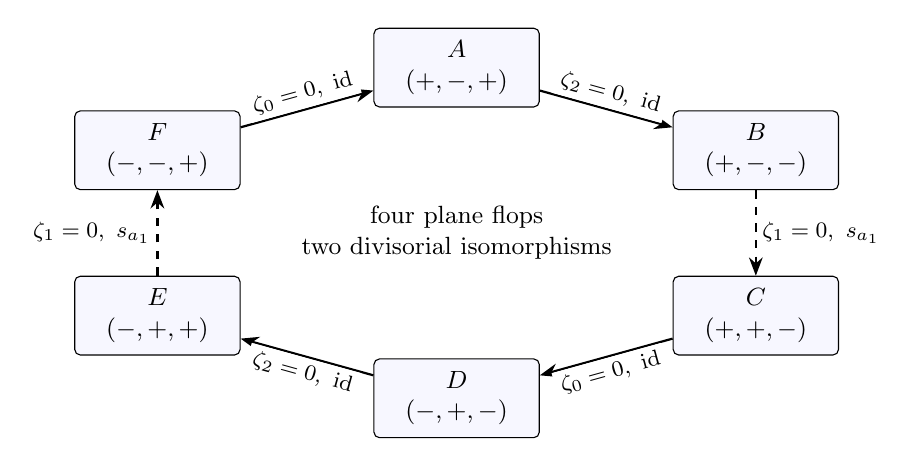
\begin{tikzpicture}[>=Stealth,
 chamber/.style={draw,rounded corners=2pt,fill=blue!3,align=center,
 minimum width=21mm,minimum height=10mm,font=\small},
 wall/.style={font=\footnotesize,fill=white,inner sep=2pt}]
\node[chamber] (A) at (0,2.1) {$A$\\$(+,-,+)$};
\node[chamber] (B) at (3.8,1.05) {$B$\\$(+,-,-)$};
\node[chamber] (C) at (3.8,-1.05) {$C$\\$(+,+,-)$};
\node[chamber] (D) at (0,-2.1) {$D$\\$(-,+,-)$};
\node[chamber] (E) at (-3.8,-1.05) {$E$\\$(-,+,+)$};
\node[chamber] (F) at (-3.8,1.05) {$F$\\$(-,-,+)$};
\draw[->,thick] (A) -- node[wall,above,sloped] {$\zeta_2=0,\ \id$} (B);
\draw[->,thick,dashed] (B) -- node[wall,right] {$\zeta_1=0,\ s_{a_1}$} (C);
\draw[->,thick] (C) -- node[wall,below,sloped] {$\zeta_0=0,\ \id$} (D);
\draw[->,thick] (D) -- node[wall,below,sloped] {$\zeta_2=0,\ \id$} (E);
\draw[->,thick,dashed] (E) -- node[wall,left] {$\zeta_1=0,\ s_{a_1}$} (F);
\draw[->,thick] (F) -- node[wall,above,sloped] {$\zeta_0=0,\ \id$} (A);
\node[align=center,font=\small] at (0,0) {four plane flops\\two divisorial isomorphisms};
\end{tikzpicture}

\end{adjustbox}
\caption{The chamber adjacency cycle. Solid edges are elementary
Mukai flops with their corrected cohomology correspondences; dashed
edges are the divisorial isomorphisms. The edge labels give the
vanishing coordinate and the Mukai action.}
\label{fig:chambers}
\end{figure}

\begin{table}[htbp]
\caption{Effective deepest surfaces and curves. In a ruled row the
last three entries are the plane line, the common negative section,
and the ruling. Here $f=c_0+c_2$.}
\label{tab:cycles}
\centering
\begin{adjustbox}{max width=\textwidth,center}
\begin{tabular}{cccl}
\toprule
Chamber & Signs $(\zeta_0,\zeta_1,\zeta_2)$ & Surfaces & Curves\\
\midrule
$A$ & $(+,-,+)$ & $p_0,p_2$ & $c_0,c_2$ (two planes)\\
$B$ & $(+,-,-)$ & $p_2,p_0-p_2$ & $-c_2;\ -c_2;\ f$\\
$C$ & $(+,+,-)$ & $p_0,p_2-p_0$ & $c_0;\ c_0;\ -f$\\
$D$ & $(-,+,-)$ & $p_0,p_2$ & $-c_0,-c_2$ (two planes)\\
$E$ & $(-,+,+)$ & $p_2,p_0-p_2$ & $c_2;\ c_2;\ -f$\\
$F$ & $(-,-,+)$ & $p_0,p_2-p_0$ & $-c_0;\ -c_0;\ f$\\
\bottomrule
\end{tabular}
\end{adjustbox}
\end{table}

Here is the geometric calculation of the table. If $P_2$ is
flopped, its graph image is $-2[P_2']$ and the exceptional
product contributes $3[P_2']$; see
\cite[Example~6.6]{llw} or \cite[\S6]{riess}. Thus the
corrected image is $[P_2']$. The other plane meets $P_2$
transversely once. Its graph image is its blow-up at that
point, and the product term adds $[P_2']$. Consequently
\begin{equation}\label{eq:surface-transform}
 p_2\longmapsto[P_2'],\qquad
 p_0\longmapsto[\Sigma]+[P_2'],\qquad \Sigma\simeq\FF_1.
\end{equation}
The common plane line and negative section represent $-c_2$.
A line in $P_0$ missing the blown-up point keeps its class;
on $\FF_1$ it is the sum of negative section and ruling.
The ruling therefore has class $f=c_0+c_2$. This gives row
$B$ and the intersection matrix
\begin{equation}\label{eq:ruled-matrix}
 \begin{pmatrix}p_2^2&p_2(p_0-p_2)\\
 p_2(p_0-p_2)&(p_0-p_2)^2\end{pmatrix}
 =\begin{pmatrix}3&-2\\-2&4\end{pmatrix}.
\end{equation}
The reflection sends $c_0$ to $-c_2$, $c_2$ to $-c_0$,
and $f$ to $-f$; it exchanges $p_0,p_2$ and preserves the
tangent Chern class. This proves row $C$. The next flop
gives the two-plane row $D$, with both line signs reversed.
Repeating gives $E,F$ and returns to $A$.

\begin{figure}[htbp]
\centering
\begin{adjustbox}{max width=\textwidth,center}
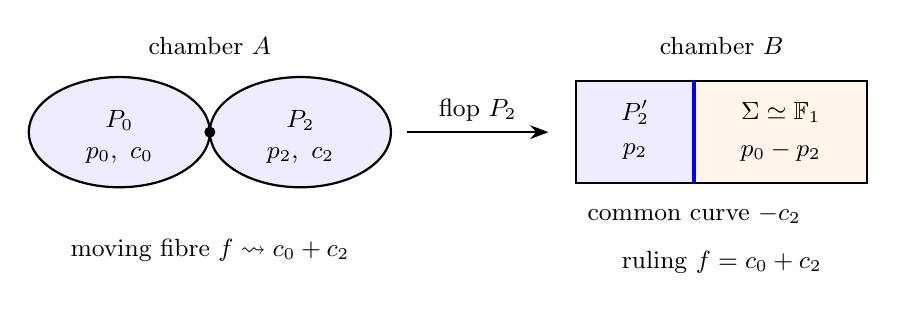
\begin{tikzpicture}[>=Stealth,font=\small]
\draw[fill=blue!7,thick] (-4,0) ellipse (1.15 and .7);
\draw[fill=blue!7,thick] (-1.7,0) ellipse (1.15 and .7);
\fill (-2.85,0) circle (2pt);
\node at (-4,0.15) {$P_0$};\node at (-1.7,0.15) {$P_2$};
\node at (-4,-.3) {$p_0,\ c_0$};\node at (-1.7,-.3) {$p_2,\ c_2$};
\node at (-2.85,1.1) {chamber $A$};
\draw[->,thick] (-.35,0) -- node[above] {flop $P_2$} (1.45,0);
\draw[fill=blue!7,thick] (1.8,-.65) rectangle (3.3,.65);
\draw[fill=orange!8,thick] (3.3,-.65) rectangle (5.5,.65);
\draw[very thick,blue] (3.3,-.65) -- (3.3,.65);
\node at (2.55,.25) {$P_2'$};\node at (2.55,-.25) {$p_2$};
\node at (4.4,.25) {$\Sigma\simeq\FF_1$};\node at (4.4,-.25) {$p_0-p_2$};
\node at (3.65,1.1) {chamber $B$};
\node[align=center] at (3.3,-1.05) {common curve $-c_2$};
\node[align=center] at (-2.85,-1.5) {moving fibre $f\rightsquigarrow c_0+c_2$};
\node[align=center] at (3.65,-1.65) {ruling $f=c_0+c_2$};
\end{tikzpicture}

\end{adjustbox}
\caption{The two configurations and their classes across the flop
from $A$ to $B$. The right-hand common curve is a line in $P_2'$
and the negative section of $\Sigma$. The moving fibre specializes
in $A$ to the reduced sum $c_0+c_2$; in $B$ this class is the
ruling of $\Sigma$. The drawings indicate incidences and cycle
classes, not metric shapes.}
\label{fig:configurations}
\end{figure}

\begin{corollary}\label{cor:gallery}
The chosen cohomological correspondences along any two paths in
the six-chamber adjacency graph with the same endpoints agree.
The complements $V_\sigma$ are isomorphic over $Z\setminus\{o\}$,
and the wall actions induce their cohomology identifications.
\end{corollary}

\begin{proof}
The six forward actions in the Mukai marking are
$\id,s_{a_1},\id,\id,s_{a_1},\id$. Their product is the identity.
Each reverse edge is the inverse correspondence. Cancellation
of reverse edges and insertion of complete six-cycles generate
the relations between paths in this graph. The ring assertion
follows. For the complements, the central map is an isomorphism
over $U$ and has the unique relative minimal $A_1$ resolution
along $S^\circ$. The local identifications agree on the dense
regular locus and glue over $Z\setminus\{o\}$.
\end{proof}

The corollary concerns these ordinary cohomological actions. It
does not identify compositions of Chow correspondences or derived
functors, and it is not a monodromy calculation for a smoothing.

\section{Integral coordinates and universal classes}\label{sec:ring}

We now give the integral coordinates in which the compact wall and
attachment calculations can be performed. The Hilbert-square basis
and Markman transport are classical inputs. The purpose of this
section is to fix their signs and the universal normalization for
this moduli problem, including arbitrary topological index classes.

\subsection{The diagonal construction}
Let $\alpha_1,\ldots,\alpha_{22}$ be an integral basis of $\Lambda$,
write $q_{ij}=\alpha_i\cdot\alpha_j$, and let $(q^{ij})$ be its
inverse matrix. Let $x_X$ be the oriented point class of $X$.
Consider
\[
 b:B=\Bl_\Delta(X\times X)\longrightarrow X\times X,
 \qquad p:B\longrightarrow Y=X^{[2]}.
\]
The map $p$ is the double cover ramified along the exceptional
divisor $E_B$. Write $j:E_B\to B$, $\pi:E_B\to X$ and
$e=[E_B]=p^*\delta$. A tensor class below is pulled back by $b$,
and $e\alpha$ means $j_*\pi^*\alpha$. The blow-up relations are
\begin{equation}\label{eq:blowup}
 \begin{gathered}
 (e\alpha)(u\otimes v)=e(\alpha uv),\qquad
 (e\alpha)(e\beta)=-[\Delta](\alpha\beta\otimes1),\\
 [\Delta]=x_X\otimes1+1\otimes x_X+
             \sum_{i,j}q^{ij}\alpha_i\otimes\alpha_j.
 \end{gathered}
\end{equation}
For the sign, $E_B|_{E_B}=-\xi$ and the excess formula gives
$b^*[\Delta]=j_*\xi$, since $c_1(TX)=0$. Hence $e^2=-b^*[\Delta]$.
In particular $e^4=24x_X\otimes x_X$. Integration on $Y$ is half
integration of a pullback on $B$; $p^*[\pt]=2x_X\otimes x_X$.
Thus \eqref{eq:blowup} is a multiplication rule using only the
marked K3 pairing.

The pullback of $\mu(\alpha)$ is $\alpha\otimes1+1\otimes\alpha$.
The classes $\mu_i=\mu(\alpha_i)$ and $\delta$ form an integral
basis in degree two. We extend $q$ to their Beauville--Bogomolov
pairing by
\begin{equation}\label{eq:BB}
 q(\mu(a),\mu(b))=q(a,b),\quad q(\mu(a),\delta)=0,\quad
 q(\delta,\delta)=-2.
\end{equation}
An integral degree-four basis consists of the classes whose
pullbacks are
\begin{equation}\label{eq:basis4}
 \begin{aligned}
 p^*A&=x_X\otimes1+1\otimes x_X,\qquad &p^*T_i&=2e\alpha_i,\\
 p^*C_{ij}&=\alpha_i\otimes\alpha_j+\alpha_j\otimes\alpha_i
       \quad(i<j),&p^*Q_i&=\alpha_i\otimes\alpha_i-e\alpha_i.
 \end{aligned}
\end{equation}
Integrality is Qin--Wang's theorem, with its K3 extension
\cite[Theorem~5.4 and Remark~5.6]{qw}, in the geometric
Nakajima conventions of \cite[Remark~5.7]{bns}. In particular
$Q_i$ is the half difference of the two Nakajima terms, not
half a symmetric square by itself. These statements apply to
all of $\Lambda$, including its nonalgebraic classes.
We use the basis statement in that reference; the product
signs here follow directly from \eqref{eq:blowup}.

For completeness we print the entire middle pairing. Degree-eight
products in the following display denote their integral against $Y$:
\begin{equation}\label{eq:gram}
 \begin{aligned}
 A^2&=1,& AT_i=AC_{ij}=AQ_i&=0,\\
 T_iT_j&=-2q_{ij},& T_iQ_j&=q_{ij},&T_iC_{jk}&=0,\\
 Q_iQ_j&=(q_{ij}^2-q_{ij})/2,&&&Q_iC_{jk}&=q_{ij}q_{ik},\\
 C_{ij}C_{kl}&=q_{ik}q_{jl}+q_{il}q_{jk}.
 \end{aligned}
\end{equation}
Every entry follows by multiplication on $B$ and division by two.
The pairing is unimodular. Eliminate the $T$ block $-2q$ over
$\Q$. Its Schur complement is half the tensor-product pairing
on the symmetric tensors in $\Lambda\otimes\Lambda$; its
determinant is $2^{-22}(\det q)^{23}$. To verify this identity,
diagonalize $q$ over a field extension: the diagonal symmetric
tensors have entries $d_i^2/2$, and the off-diagonal ones have
entries $d_i d_j$. The product is the stated expression, and
the identity descends over $\Q$. The determinant of the whole
pairing is therefore
$\det(-2q)2^{-22}(\det q)^{23}=(\det q)^{24}=1$.
This also verifies index one, once integrality and the known
free rank $276$ are supplied.

Products of degree-two classes are
\begin{equation}\label{eq:degree2-products}
 \begin{aligned}
 \mu_i\mu_j&=q_{ij}A+C_{ij} &&(i<j),\\
 \mu_i^2&=q_{ii}A+2Q_i+T_i,&\mu_i\delta&=T_i,\\
 \delta^2&=-A-\sum_iq^{ii}Q_i-\tfrac12\sum_iq^{ii}T_i
                     -\sum_{i<j}q^{ij}C_{ij}.
 \end{aligned}
\end{equation}
The diagonal of $q^{-1}$ is even because the dual K3 lattice is
even. Thus the last expression is integral. If $\alpha^i$ is the
$q$-dual basis, set
\begin{equation}\label{eq:basis6}
 R_i=\mu(\alpha^i)A,\qquad R_\delta=-\delta A.
\end{equation}
These classes are dual to $\mu_i,\delta$ and form an integral
degree-six basis. For $a\in R^2$ and $z\in R^4$, its product
$az$ has coefficient $\int_Y\mu_i az$ on $R_i$ and
$\int_Y\delta az$ on $R_\delta$. These are given by
\eqref{eq:degree2-products} and \eqref{eq:gram}.
Together with the unit, the oriented point, the dual degree-two/
degree-six pairing, and zero odd groups, this specifies every product.
The ranks are $1,23,276,23,1$. Torsion-freeness is the integral
Hilbert-scheme theorem; see \cite[Theorem~3.1]{totaro}.

The formulas also exhibit rational generation by degree two:
\begin{equation}\label{eq:rational-generation}
 A=\frac1{10}\delta^2+\frac1{20}\sum_{i,j}q^{ij}\mu_i\mu_j,
\end{equation}
after which \eqref{eq:degree2-products} gives $T_i,C_{ij},Q_i$,
and \eqref{eq:basis6} gives degree six. The integral ring generally
requires more than the integral symmetric square.

We will also use the classical tangent-class identity
\begin{equation}\label{eq:c2}
 c_2(Y)=24A-3\delta^2
\end{equation}
of Shen--Vial \cite[Lemma~14.4]{sv}. Their incidence-surface
class is $A$ here. Their rational Chow identity gives this integral
cohomological identity by torsion-freeness. The preceding products
give, independently,
\[
 \int_Y\delta^4=12,\quad
 \int_Y c_2\mu(a)\mu(b)=30q(a,b),\quad
 \int_Yc_2\delta^2=-60,\quad \int_Yc_2^2=828.
\]

\subsection{Transport from the rank-three moduli}
Set $a_H=(1,H,2)$, $C_0=D_1+D_2-2H$ and
\begin{equation}\label{eq:g}
 g=e^{-C_0}s_{a_H},\qquad s_{a_H}(z)=z+(z,a_H)a_H.
\end{equation}
Here $e^D(r,c,s)=(r,c+rD,s+cD+rD^2/2)$.
The input lattice gives
\[
 a_H^2=-2,\quad (v,a_H)=-2,\quad C_0^2=-14,\quad
 s_{a_H}(v)=(1,C_0,-8),\quad g(v)=v'=(1,0,-1).
\]
This is the integral Mukai isometry induced by the spherical twist
about $\OO_X(H)$ followed by tensoring with $\OO_X(-C_0)$.
It need not send each chamber sheaf to a sheaf.

The polarizations may be chosen in each sector with degree coprime
to three, as in \cite[\S4.5]{wuebben17}; the full compact
Gieseker moduli therefore satisfies Markman's suitability condition
\cite[Definition~3.4]{markman08}. His universal Chern
correspondence \cite[Theorem~1.2 and equation~(3)]{markman08}
gives
\begin{equation}\label{eq:Phi}
 \Phi_\sigma=\gamma_{g,v}:H^*(M_\sigma,\Z)\xrightarrow{\sim} R.
\end{equation}
The source and target are torsion-free: for the source use the
K3$^{[2]}$ deformation type established in Section~\ref{sec:geometry},
and for the Hilbert square use \cite[Theorem~3.1]{totaro}.
Thus the modulo-torsion qualification loses nothing here.
The correspondence preserves tangent Chern classes and
orientation; for the latter, preservation of $c_4=324[\pt]$
suffices. Compatibility with the Mukai homomorphisms is
\cite[Theorem~3.9 and diagram~(41)]{markman08}:
\begin{equation}\label{eq:theta-transport}
 \Phi_\sigma\theta_v(z)=\theta_{v'}(gz),\qquad
 \theta_{v'}(r,c,r)=\mu(c)+r\delta.
\end{equation}
The sign in the second formula follows from the universal ideal
sequence: $c_1(\OO_X^{[2]})=-\delta$, while the index of
$(r,-c,r)$ is its Euler characteristic minus its tautological
class. This determines $\Phi_\sigma$ without choosing an
unspecified deformation path.

\subsection{Topological indices and determinant normalization}
Let $\mathcal I$ be the universal ideal class on $X\times Y$.
For a topological class $F$ let $F^{[2]}$ denote the index
defined by the universal length-two subscheme. With $g$ acting
on topological classes through their Mukai vectors, put
\begin{equation}\label{eq:J}
 J_z=\chi_X((gz)^\vee)\,1-((gz)^\vee)^{[2]},\qquad
 \mathcal L=\det J_y,\qquad \widehat J_z=J_z\otimes\mathcal L^{-1}.
\end{equation}
Here $gy=(0,-f_2,1)$ and $\rank J_y=1$.

\begin{proposition}\label{prop:indices}
For every $z\in K^0_{\mathrm{top}}(X)$ and $k\ge0$,
\begin{equation}\label{eq:indices-transport}
 \Phi_\sigma(c_k(I_z^y))=c_k(\widehat J_z).
\end{equation}
These classes are calculated in the integral basis above by
\begin{equation}\label{eq:tautological-character}
 p^*\ch(F^{[2]})=\ch(F)_1e^{-e}+\ch(F)_2,
 \qquad F\in K^0_{\mathrm{top}}(X).
\end{equation}
Subscripts denote the two pullbacks from $X$ to $B$.
\end{proposition}

\begin{proof}
Markman's universal-class identity intertwines the universal Chern
characters up to a topological base line bundle. Contract its K3
factor against $gz$ using the Euler pairing. Since $g$ is an
Euler isometry, the index characters are intertwined up to that
same line. Taking the determinant of the rank-one $y$-index
multiplies it by exactly this line, so normalization cancels it.
The resulting normalized characters agree over $\Q$, and hence
so do the Chern classes. Both Chern classes are integral and
$H^*(Y,\Z)$ is torsion-free, proving
\eqref{eq:indices-transport} integrally.

We prove \eqref{eq:tautological-character} for topological $F$,
without requiring an algebraic representative of its first
Chern class. Let $\mathcal Z\subset Y\times X$ be the
universal subscheme and pull it back to $\mathcal Z_B\subset
B\times X$. The incidence description is the diagonal blow-up
\cite[\S10, diagram~(54)]{sv}. If $q_1,q_2:B\to X$
are the projections, $\mathcal Z_B$ is the scheme-theoretic
union of their graphs, intersecting in the graph over $E_B$.
This includes the nonreduced fibre: in a blow-up chart with
difference coordinates $(t,tw)$ the length-two algebra is
$A[U]/(U(U-t))$. Evaluation at $0,t$ maps it injectively to
$A\oplus A$, with image the pairs agreeing modulo $t$ and
cokernel $A/(t)$. The other blow-up chart gives the same
description. Thus there is an exact sequence of kernels
\begin{equation}\label{eq:kernel}
 0\longrightarrow\OO_{\mathcal Z_B}\longrightarrow
 \OO_{\Gamma_1}\oplus\OO_{\Gamma_2}\longrightarrow
 \OO_{\Gamma_{E_B}}\longrightarrow0.
\end{equation}
All these kernels are perfect on the smooth product $B\times X$.
Pass their equality to topological $K$-theory, tensor with the
pullback of any $F$, and push forward to $B$. Base change for
the complex-oriented projection and functoriality give
\[
 p^*F^{[2]}=q_1^*F+q_2^*F-j_!\pi^*F
           =q_1^*F\otimes\OO_B(-E_B)+q_2^*F.
\]
The last equality uses the divisor Koszul class
$j_!1=1-[\OO_B(-E_B)]$ and the projection formula. Only the
fixed kernel in \eqref{eq:kernel} needed an algebraic
representative. The equality therefore holds for arbitrary
topological $F$. Applying the Chern character proves
\eqref{eq:tautological-character}.
\end{proof}

For use as a finite formula, a Mukai vector $(r,c,s)$ has
ordinary character $r+c+(s-r)x_X$. Truncate the exponential
in \eqref{eq:tautological-character} after degree eight,
form \eqref{eq:J}, and multiply its character by
$\exp(-c_1(J_y))$. The Newton identities recover $c_1$ through
$c_4$; higher classes vanish on $Y$. Formula
\eqref{eq:blowup} and the integral bases then give their
coordinates. This covers virtual classes of every rank.
The intermediate arithmetic is rational, but the results are
Chern classes of integral topological indices.

\subsection{Exceptional coordinates}
Applying \eqref{eq:g} to \eqref{eq:curves} gives
\begin{equation}\label{eq:gc}
 gc_0=(5/2,u_0,5/2),\qquad
 gc_2=(-3/2,u_2,-3/2),\qquad q(u_0)=10,\quad q(u_2)=2.
\end{equation}
Substituting \eqref{eq:theta-transport} and \eqref{eq:c2}
in the plane formula gives exactly
\eqref{eq:planes-intro}. For any $a\in\Lambda$,
$\mu(a)^2-\delta\mu(a)$ is even by
\eqref{eq:degree2-products} and the evenness of $q$.
This proves the asserted integrality of both plane coordinates.
Multiplication gives $p_0^2=p_2^2=3$ and $p_0p_2=1$.

Write
\begin{equation}\label{eq:d-ell}
 \begin{gathered}
 \lambda_0=\mu(u_0)+\tfrac52\delta,\qquad
 \lambda_2=\mu(u_2)-\tfrac32\delta,\qquad d_i(a)=q(\lambda_i,a),\\
 \ell_0=\sum_jq(u_0,\alpha_j)R_j-5R_\delta,\qquad
 \ell_2=\sum_jq(u_2,\alpha_j)R_j+3R_\delta.
 \end{gathered}
\end{equation}
The functionals $d_i:R^2\to\Z$ are integral, and $\ell_i$
is their Poincar\'e dual. They are precisely the line
functionals and line classes of the two planes under $\Phi_A$.
The primitive witnesses \eqref{eq:witness-restrictions}
therefore apply to these explicit coordinates.

\section{The complement and its integral attachments}\label{sec:attachments}

All coordinates in this section refer to the ring $R$ of
Section~\ref{sec:ring}. In particular the ambient multiplication
and the exceptional classes have already been calculated. We use
excision to determine the complement and its maps, with integral
coefficients throughout.

\subsection{The exceptional ideal}
First work in chamber $A$, with $E=P_0\cup P_2$ and $V=M_A\setminus E$.
The planes meet at one point, so a regular neighborhood retracts
to $\PP^2\vee\PP^2$. Integral Poincar\'e--Lefschetz duality on the regular neighborhood,
followed by excision \cite[Theorem~3.43]{hatcher}, gives
\begin{equation}\label{eq:relative}
 H^k(M_A,V)\simeq H_{8-k}(E).
\end{equation}
The only nonzero relative groups are in degrees $4,6,8$, with
ranks $2,2,1$. Their maps to the absolute cohomology are the
plane, line and point inclusions, respectively.

\begin{proposition}\label{prop:complement}
Restriction is a surjective ring homomorphism with kernel
$(p_0,p_2)$. Hence $H^*(V,\Z)=R/(p_0,p_2)$, with free ranks
$1,23,274,21$ in degrees $0,2,4,6$ and no other groups.
\end{proposition}

\begin{proof}
The witnesses \eqref{eq:witness-restrictions} show that the
relative plane and line maps in \eqref{eq:relative} are
primitive injections. The point map is an isomorphism. The
long exact sequence of the pair therefore gives surjectivity
of restriction, vanishing of odd groups, and the stated free
quotients. It remains to identify its kernel as an ideal,
rather than merely as three additive subgroups.

The projection formula on the two planes gives
\begin{equation}\label{eq:ideal-products}
 p_i a=d_i(a)\ell_i\quad(a\in R^2),\qquad
 p_i z=\left(\int_Yp_i z\right)[\pt]\quad(z\in R^4).
\end{equation}
Each $d_i$ takes the value one, and each plane evaluation
takes the value one, by the same unimodular witnesses. Thus
the ideal contains $\ell_0,\ell_2$ and $[\pt]$. Its degree-four
part is exactly the span of $p_0,p_2$ and it has no further
possible degrees. This is the entire restriction kernel
computed from \eqref{eq:relative}, proving the ring statement.
\end{proof}

For every normalized index, restriction to $V$ is consequently
the class $c_k(\widehat J_z)$ of Proposition~\ref{prop:indices}
reduced modulo this explicit ideal. No complement multiplication
is an additional input to that formula.

\subsection{The two-plane neighborhood and its boundary}
Choose a smoothed closed regular neighborhood $W$ of $E$ and
put $L=\partial W$, with the outward boundary orientation from
the complex orientation of $W$. It is the plumbing of the
cotangent normal disk bundles of the two planes. Their normal
Euler numbers are three and their transverse intersection is
positive one. The middle intersection matrix is therefore
\begin{equation}\label{eq:B}
 B=\begin{pmatrix}3&1\\1&3\end{pmatrix}.
\end{equation}
A deleted collar retracts to $L$, so $L$ models the actual
overlap in the cover of $M_A$ by $V$ and an open enlargement
of $W$. It is a boundary inside the resolution. The singular
surface of the target passes through $o$; $L$ is not the link
of an isolated target singularity.

Let $h_i$ be the positive hyperplane classes of the two
components and $t_i=h_i^2$. The neighborhood ring is the
wedge ring
\begin{equation}\label{eq:W-ring}
 h_0h_2=0,\qquad h_i^2=t_i,
\end{equation}
with all products of degree greater than four zero.
Restriction from $R$ is
\begin{equation}\label{eq:W-restrictions}
 a\longmapsto d_0(a)h_0+d_2(a)h_2,\qquad
 z\longmapsto\left(\int_Yzp_0\right)t_0+
                    \left(\int_Yzp_2\right)t_2
\end{equation}
in degrees two and four. It preserves the unit and is zero
in higher positive degrees.

The Poincar\'e--Lefschetz sequence for $(W,L)$ gives
\begin{equation}\label{eq:L-groups}
 H^k(L,\Z)=
 \begin{cases}
 \Z,&k=0,7,\\
 \Z^2,&k=2,5,\\
 \Z/8,&k=4,\\
 0,&\text{otherwise}.
 \end{cases}
\end{equation}
Indeed its only nontrivial even map in the middle is $B$,
whose determinant is eight and whose entries have gcd one.
The quotient map $\Z^2/B\Z^2\to\Z/8$ is
$(n_0,n_2)\mapsto n_0-3n_2$.
Write $x_i$ for the images of $h_i$ and $\tau$ for the
image of $t_0$. If $\omega$ is the oriented degree-seven
generator, choose $\eta_0,\eta_2\in H^5(L,\Z)$ dual to $x_0,x_2$.
The complete nonzero positive products are
\begin{equation}\label{eq:L-products}
 x_0^2=\tau,\quad x_2^2=-3\tau,\quad
 x_i \eta_j=\delta_{ij}\omega,\qquad 8\tau=0,
\end{equation}
and $x_0x_2=0$. Degree and \eqref{eq:L-groups} make all
other positive products zero. The free pairings follow from
oriented Poincar\'e duality; the torsion products follow by
restricting \eqref{eq:W-ring}. These statements describe the
ordinary ring, without asserting an additional torsion linking form.

\begin{proposition}\label{prop:boundary}
With the preceding choices, restriction $\rho:H^*(V)\to H^*(L)$
is
\begin{equation}\label{eq:rho}
 \rho^2(a)=d_0(a)x_0+d_2(a)x_2,\qquad
 \rho^4([z])=\kappa([z])\tau,\quad
 \kappa([z])=\int_Yz(p_0-3p_2)\pmod8.
\end{equation}
It preserves the unit, and its other positive-degree maps vanish.
For the ordered cover $(V,W)$ with alternating map $r_V-r_W$,
the Mayer--Vietoris connecting homomorphisms are
\begin{equation}\label{eq:MV}
 \partial_{\mathrm{MV}}\eta_i=-\ell_i,\qquad
 \partial_{\mathrm{MV}}\omega=-[\pt].
\end{equation}
\end{proposition}

\begin{proof}
Restrictions from $M_A$ to the overlap agree whether taken
through $V$ or $W$. Surjectivity in
Proposition~\ref{prop:complement} and
\eqref{eq:W-restrictions} therefore give \eqref{eq:rho}.
It is well-defined: evaluation of $p_0-3p_2$ against
$p_0,p_2$ gives $0,-8$. Multiplicativity may also be checked
without referring back to the geometric map. For $a,b\in R^2$,
\[
 \int_Yabp_i=d_i(a)d_i(b),
\]
which is exactly the product prescribed by
\eqref{eq:L-products}. All further positive products have
zero target. This checks the map on the complete integral
basis and every ring relation.

For signs, the pair boundary of $(W,L)$ sends the degree-five
classes dual to $h_i$ to the positive relative line classes,
and its oriented top class to the positive relative point
class, by Stokes' convention with outward boundary. Excision
identifies their images in $M_A$ with $\ell_i,[\pt]$.
In the ordered alternating restriction $r_V-r_W$, a
cochain supported on the $W$ side has the negative of that
pair boundary. This yields \eqref{eq:MV}.
\end{proof}

\begin{figure}[htbp]
\centering
\begin{adjustbox}{max width=\textwidth,center}
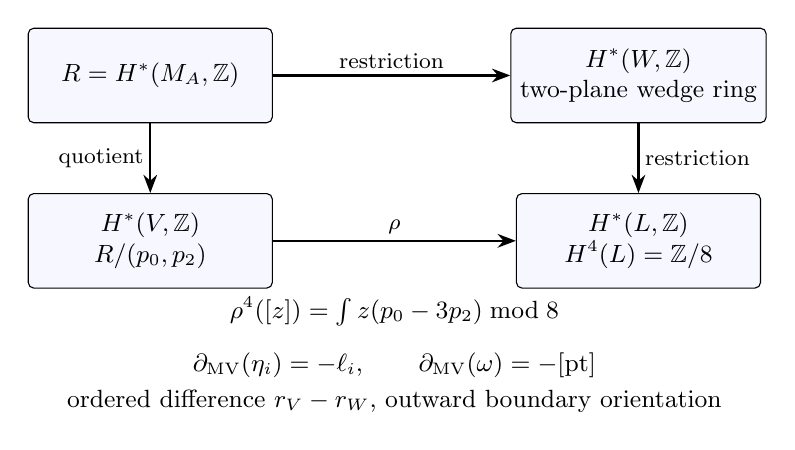
\begin{tikzpicture}[>=Stealth,font=\small,
 box/.style={draw,rounded corners=2pt,fill=blue!3,align=center,
             minimum height=12mm,minimum width=31mm},
 label/.style={fill=white,inner sep=2pt,font=\footnotesize}]
\node[box] (M) at (0,0) {$R=H^*(M_A,\Z)$};
\node[box] (W) at (6.2,0) {$H^*(W,\Z)$\\two-plane wedge ring};
\node[box] (V) at (0,-2.1) {$H^*(V,\Z)$\\$R/(p_0,p_2)$};
\node[box] (L) at (6.2,-2.1) {$H^*(L,\Z)$\\$H^4(L)=\Z/8$};
\draw[->,thick] (M) -- node[label,above] {restriction} (W);
\draw[->,thick] (M) -- node[label,left] {quotient} (V);
\draw[->,thick] (W) -- node[label,right] {restriction} (L);
\draw[->,thick] (V) -- node[label,above] {$\rho$} (L);
\node at (3.1,-3.0) {$\rho^4([z])=\int z(p_0-3p_2)\bmod8$};
\node[align=center] at (3.1,-3.9)
 {$\partial_{\rm MV}(\eta_i)=-\ell_i,\qquad
   \partial_{\rm MV}(\omega)=-[\mathrm{pt}]$\\[2pt]
  ordered difference $r_V-r_W$, outward boundary orientation};
\end{tikzpicture}

\end{adjustbox}
\caption{The computed restriction square in chamber $A$.
The lower map in degree four is $\kappa$ and the right map
is the cokernel of $B$. The signed connecting maps belong
to the ordered Mayer--Vietoris sequence and are separate
from these ring homomorphisms.}
\label{fig:excision}
\end{figure}

In degree four the square recovers the additive compatibility
description
\begin{equation}\label{eq:fiber-product}
 R^4\simeq
 \left\{([z],n_0,n_2):\ n_0-3n_2\equiv
          \int_Yz(p_0-3p_2)\pmod8\right\},
\end{equation}
where $[z]\in(R/(p_0,p_2))^4$. The ambient ring was already
constructed in Section~\ref{sec:ring};
\eqref{eq:fiber-product} is not a separate derivation of
multiplication from an additive sequence.

For the normalized indices, \eqref{eq:index-plane} gives
\begin{equation}\label{eq:index-kappa}
 \begin{aligned}
 \kappa(c_2(I_z^y))&=\binom{m_0(z)}2-3\binom{m_2(z)}2\pmod8,\\
 \kappa(c_1(I_z^y)c_1(I_{z'}^y))
     &=m_0(z)m_0(z')-3m_2(z)m_2(z')\pmod8.
 \end{aligned}
\end{equation}
These reproduce the earlier binomial attachment of
\cite[\S6.4]{wuebben17}. The present formula also calculates
its full domain: evaluate on $A,T_i,C_{ij},Q_i$ using
\eqref{eq:gram}, with $p_i$ expanded by
\eqref{eq:degree2-products}. This is a specified integral
generating set with all its products, not a test on a
possibly proper sublattice of degree four.

\subsection{A uniform formula for all six chambers}
In chamber $D$ the two planes have the same surface classes
and the negative line classes. Thus use the preceding formulas
with degree-two restriction $a\mapsto\epsilon d_0(a)h_0+
\epsilon d_2(a)h_2$, where $\epsilon=1$ in $A$ and $-1$ in
$D$. The relative maps in degrees $4,6,8$ are
\begin{equation}\label{eq:two-plane-relative}
 (p_0,p_2),\qquad (\epsilon\ell_0,\epsilon\ell_2),\qquad[\pt].
\end{equation}
The boundary ring and degree-four functional are unchanged,
and the connecting maps are the negatives of the displayed
line and point maps.

For the four ruled configurations use
\begin{equation}\label{eq:ruled-template}
 \begin{array}{c|rrrr}
 \sigma&B&C&E&F\\\hline
 (k,j,\epsilon)&(2,0,-1)&(0,2,1)&(2,0,1)&(0,2,-1).
 \end{array}
\end{equation}
The surfaces are $p_k$ and $p_j-p_k$. Write $e_\Sigma$ for
the negative section and $r_\Sigma$ for the ruling in
$\Sigma\simeq\FF_1$. Their global curve classes are
\begin{equation}\label{eq:ruled-curves}
 [e_\Sigma]=\epsilon c_k,\qquad
 [r_\Sigma]=-\epsilon(c_0+c_2),\qquad
 e_\Sigma^2=-1,\quad e_\Sigma r_\Sigma=1,\quad r_\Sigma^2=0.
\end{equation}
Let $\xi,\upsilon\in H^2(W_\sigma)$ take values $(1,0)$
and $(0,1)$ on $(e_\Sigma,r_\Sigma)$. Their restrictions
to the plane are $h,0$ and to $\Sigma$ are
$r_\Sigma,e_\Sigma+r_\Sigma$, respectively. With
$t_P,t_\Sigma$ dual to the two surface components, the ring is
\begin{equation}\label{eq:ruled-W}
 \xi^2=t_P,\qquad \xi\upsilon=\upsilon^2=t_\Sigma,
\end{equation}
with higher positive products zero. This follows from the
Mayer--Vietoris ring of the two components meeting along
their common curve, or directly from the two restrictions.

For $a\in R^2$ set $s=\epsilon d_k(a)$ and
$t=-\epsilon(d_0(a)+d_2(a))$. The complete positive
restrictions to the neighborhood are
\begin{equation}\label{eq:ruled-restriction}
 \begin{aligned}
 a|_{W_\sigma}&=s\xi+t\upsilon,&
 a|_\Sigma&=t e_\Sigma+(s+t)r_\Sigma,\\
 z|_{W_\sigma}&=\left(\int_Yzp_k\right)t_P+
                   \left(\int_Yz(p_j-p_k)\right)t_\Sigma.
 \end{aligned}
\end{equation}
The relative middle matrix is
$B'=\bigl(\begin{smallmatrix}3&-2\\-2&4\end{smallmatrix}\bigr)$
from \eqref{eq:ruled-matrix}. Its cokernel map is
$(n_P,n_\Sigma)\mapsto6n_P+n_\Sigma\pmod8$.
The boundary has the groups \eqref{eq:L-groups}.
Write $\tau_k$ for the image of $t_\Sigma$ and retain the
symbols $\xi,\upsilon$ for their boundary images. Its nonzero
positive products are
\begin{equation}\label{eq:ruled-L}
 \xi^2=6\tau_k,\quad \xi\upsilon=\upsilon^2=\tau_k,
 \quad \xi \eta_\xi=\upsilon \eta_\upsilon=\omega,\quad8\tau_k=0,
\end{equation}
where $\eta_\xi,\eta_\upsilon$ are the dual degree-five basis.
Their cross pairings are zero. Every other positive product
vanishes.

\begin{proposition}\label{prop:all-attachments}
In every ruled row of \eqref{eq:ruled-template}, restriction
from the complement is
\begin{equation}\label{eq:ruled-rho}
 \rho^2(a)=s\xi+t\upsilon,\qquad
 \rho^4([z])=\left(\int_Yz(p_j+5p_k)\right)\tau_k\pmod8.
\end{equation}
Its relative maps in degrees $4,6,8$ are
\begin{equation}\label{eq:ruled-relative}
 (p_k,p_j-p_k),\qquad
 (\epsilon\ell_k,-\epsilon(\ell_0+\ell_2)),\qquad[\pt].
\end{equation}
For the ordered difference $r_V-r_W$, the connecting maps
on $\eta_\xi,\eta_\upsilon,\omega$ are the negatives of the
corresponding line and point maps. All six complement
rings are $R/(p_0,p_2)$.
\end{proposition}

\begin{proof}
Proposition~\ref{prop:compact-walls} and
\eqref{eq:surface-transform} give these as the actual
adjacent compact configurations. The two surface classes
generate the same ideal $(p_0,p_2)$, and their line pair
is a unimodular change of $\ell_0,\ell_2$.
The relative groups and primitive maps therefore give
the same quotient proof as in
Proposition~\ref{prop:complement}. Their regular
neighborhoods have the computed component ring and
intersection matrix, so Poincar\'e--Lefschetz duality
gives \eqref{eq:ruled-L} and \eqref{eq:ruled-rho}.
The actual compact maps identify the exteriors, and
regular levels outside the exceptional core identify
their outward boundaries. Thus these are the overlap
maps of the given geometric gluing.

To check integrality and multiplicativity explicitly,
evaluation of $p_j+5p_k$ against $p_j,p_k$ gives $8,16$,
so the degree-four map kills the ideal. For $a,b\in R^2$,
\[
 \int_Yabp_k=d_k(a)d_k(b),\qquad
 \int_Yab(p_j-p_k)=d_j(a)d_j(b)-d_k(a)d_k(b).
\]
Substitution of $s,t$ in \eqref{eq:ruled-L} gives
$6s_as_b+s_at_b+t_as_b+t_at_b$, which is the same
value modulo eight. All other positive products have
zero target. The relative maps are the geometric
component, line and point inclusions. Their connecting
signs follow from the same outward Stokes convention as
\eqref{eq:MV}.
\end{proof}

For $k=2$ the functional in \eqref{eq:ruled-rho} is
$\kappa$, while for $k=0$ it is $5\kappa$. This change
records the torsion-generator convention, not a new
uncomputed gluing choice. For example across $A\to B$,
the degree-two boundary classes transform as
\[
 x_0\longmapsto\upsilon,\qquad
 x_2\longmapsto\upsilon-\xi.
\]
The degree-five classes transform by the inverse transpose:
$\eta_0\mapsto \eta_\xi+\eta_\upsilon$, $\eta_2\mapsto-\eta_\xi$,
and $\omega\mapsto\omega$. These formulas preserve
\eqref{eq:L-products} and \eqref{eq:ruled-L}, with
$\tau\mapsto\tau_2$.

\subsection{The moving divisor remains in the complement}
The open set $V_\sigma$ contains the divisor $D^\circ$
over $S^\circ$, so it is larger than $\pi_\sigma^{-1}(U)$.
We record its established ring to make this distinction
explicit. In chamber $A$ use $x$ from \eqref{eq:witness},
set $z_D=a_1+2x$, and put
\[
 d=\theta_w(z_D)|_{S^\circ},\qquad
 h_D=\theta_v(x)|_{D^\circ}.
\]
The open-divisor calculation of \cite[\S7]{wuebben17} is
\begin{equation}\label{eq:moving-ring}
 \begin{gathered}
 H^2(S^\circ,\Z)=H^2(S,\Z)/\Z[C]\simeq\Z^{21},\qquad
 H^k(S^\circ,\Z)=0\quad(k>0,\ k\ne2),\\
 H^*(D^\circ,\Z)=H^*(S^\circ,\Z)[h_D]/(h_D^2-dh_D),\qquad
 D|_{D^\circ}=-2h_D+\pi^*d.
 \end{gathered}
\end{equation}
Here $[C]$ is primitive, so the Gysin sequence gives the
base cohomology. The $\mathrm{PGL}_2$ structure group acts
trivially on fibre cohomology, and $h_D$ has fibre degree
one, giving an integral Leray--Hirsch basis. The topological
rank-two lift exists because $H^3(S^\circ,\Z)=0$;
normalizing its hyperplane class to $h_D$ gives first
Chern class $d$ and zero second Chern class. The universal
extension gives the divisor identity; the orthogonality
of $z_D$ to $a_1,w,v$ removes base-line ambiguities.

The algebraic Brauer obstruction remains nonzero of order
two on $S^\circ$: restriction to the function field is
injective for a regular integral surface. Its analytic
image on this open surface vanishes, using
$H^2(S^\circ,\OO)=H^3(S^\circ,\Z)=0$. These lifting
statements and their primary sources are proved in
\cite[\S7.1]{wuebben17}. They do not imply an algebraic
universal family over the full compact $S$. The divisorial
wall proof used coarse blow-ups precisely so that such a
lift was unnecessary.

\section{The wall actions in integral coordinates}\label{sec:actions}

The compact geometric actions were proved in
Proposition~\ref{prop:marked-wall}. We now give their
coordinates on every degree of $R$ and on the normalized
indices. This also verifies compatibility with the
attachment formulas.

\subsection{All ring generators}
At a divisorial wall the action in $R$ is the conjugate
of $s_{a_1}$ by $g$. Put
\begin{equation}\label{eq:reflection-root}
 k_0=2H-D_2,\qquad r=\mu(k_0)+\delta
             =\theta_{v'}(ga_1),\qquad q(k_0)=0,
 \quad q(r)=-2.
\end{equation}
Write $\mathsf S$ for this integral ring automorphism. Its degree-two
action is
\begin{equation}\label{eq:S2}
 \mathsf S(\mu(b))=\mu(b)+q(b,k_0)r,\qquad \mathsf S(\delta)=\delta-2r.
\end{equation}
Set $\mu_i'=\mathsf S(\mu_i)$, $\delta'=\mathsf S(\delta)$. The full
degree-four action is
\begin{equation}\label{eq:S4}
 \begin{aligned}
 A'&=\frac{c_2(Y)+3(\delta')^2}{24}
     =A+\frac{\mu(k_0)^2+\delta\mu(k_0)}2,\\
 T_i'&=\mu_i'\delta',\qquad
 C_{ij}'=\mu_i'\mu_j'-q_{ij}A',\\
 Q_i'&=\frac{(\mu_i')^2-q_{ii}A'-T_i'}2.
 \end{aligned}
\end{equation}
In degree six the images are
$\mathsf S(R_i)=\mathsf S(\mu(\alpha^i))A'$ and
$\mathsf S(R_\delta)=-\delta'A'$. The unit and oriented point are
fixed. Formula \eqref{eq:S4} follows from preservation of
$c_2(Y)$ and \eqref{eq:degree2-products}. Its apparently
rational expressions are integral because they are images
under the integral ring map already constructed; the
second formula for $A'$ also shows its integrality
directly. These identities give a finite coordinate
calculation on the entire lattice, including the classes
outside its integral symmetric square.

They imply
\begin{equation}\label{eq:planes-reflection}
 \mathsf S(p_0)=p_2,\quad \mathsf S(p_2)=p_0,\quad \mathsf S(c_2(Y))=c_2(Y),
 \quad \mathsf S^2=\id.
\end{equation}
Consequently $\mathsf S$ preserves the exceptional ideal. In the
fixed two-plane torsion convention,
\[
 \kappa(\mathsf S z)=5\kappa(z)\pmod8,
\]
because $p_2-3p_0\equiv5(p_0-3p_2)$ modulo eight in
the integral lattice. The ruled conventions in
\eqref{eq:ruled-rho} incorporate exactly this change.
At a plane wall every generator has the identity action
in $R$, with the geometric surface change
\eqref{eq:surface-transform} still understood. It is the
exceptional product in \eqref{eq:flop-correspondence}
that makes this the action of a multiplicative
correspondence.

\subsection{The fixed determinant normalizer}
Let $h=\id$ or $s_{a_1}$ act between the source and target
Mukai lattices, and retain the original $y$ on both sides.
Markman's universal-class identity, followed by the
rank-one normalization argument, gives
\begin{equation}\label{eq:wall-indices}
 \gamma_h\bigl(c_k(I_z^y)\bigr)=
 c_k\left(I_{hz}^y\otimes(\det I_{hy}^y)^{-1}\right).
\end{equation}
Indeed transport first gives the target universal family
normalized by $hy$ rather than by $y$. Starting from the
$y$-normalized target family, its $hy$-index still has
rank one, so tensoring by its inverse determinant is
exactly that change of normalization. Equality of
characters implies equality of integral Chern classes
by torsion-freeness, as in
Proposition~\ref{prop:indices}.

For $h=\id$ the determinant is trivial. For $h=s_{a_1}$,
$(y,a_1)=-1$ and hence $hy=y-a_1$. Additivity of the
index and $\det I_y^y=1$ give
\begin{equation}\label{eq:normalizer-line}
 c_1\left((\det I_{y-a_1}^y)^{-1}\right)=\theta_v(a_1),
 \qquad \Phi\theta_v(a_1)=r.
\end{equation}
Thus in the common ring the transformed character is
$\ch(I_{s_{a_1}z}^y)\exp(r)$, not merely the character
with its input vector reflected. Formula
\eqref{eq:tautological-character} and the Newton identities
calculate all its Chern classes. Functoriality includes
these normalizing lines, so they introduce no ambiguity
in the six-step cohomological identity.

\subsection{Dependence on the choices}
An integral change of basis of $\Lambda$ changes the
coordinates in \eqref{eq:basis4} and \eqref{eq:basis6}
by the corresponding integral transformation. The
diagonal construction itself is intrinsic. The isometry
$g$ and the universal normalizer $y$ are specified:
Markman's functoriality fixes the transport, and
\eqref{eq:wall-indices} describes any change of the
normalizer. Different geometric realizations of an
action with the same degree-two marking have the same
cohomological action, by rational generation and
torsion-freeness.

Isotopic regular neighborhoods give the same restriction
and relative maps by naturality of excision. The outward
orientation and the ordered difference $r_V-r_W$ fix
the connecting signs. Replacing a torsion generator by
a unit multiple changes the printed mod-eight functional
by that unit. These choices specify the calculated
cohomology and its maps; no assertion about a homotopy
classification of the gluing follows from them.

\begin{proof}[Proof of Theorem~\ref{thm:main}]
Proposition~\ref{prop:compact-walls} constructs the
compact partial-wall maps, and
Lemma~\ref{lem:opposite-divisors} and
Proposition~\ref{prop:marked-wall} identify their
integral actions. Equations \eqref{eq:Phi}--\eqref{eq:gc}
give the specified ambient marking and exceptional
coordinates. Propositions~\ref{prop:complement},
\ref{prop:boundary} and \ref{prop:all-attachments}
calculate the complement and every attachment map.
Proposition~\ref{prop:indices} and
\eqref{eq:wall-indices} give the universal-index
markings and their determinant correction. Finally
Corollary~\ref{cor:gallery} proves the cohomological
path relation. All computations use the same compact
moduli problem and the same primitive cycles.
\end{proof}

\subsection{Exact verification}
The formulas above are finite expressions in the marked
K3 Gram matrix. Accompanying standard-library Python
programs implement \eqref{eq:blowup} with rational
arithmetic. They compute the integral middle pairing,
the two plane coordinates, the four Chern classes of
each index for a $24$-element topological $K$-basis, and
the images of every degree-two, degree-four and
degree-six basis element under $\mathsf S$. Additional virtual
classes test negative ranks and the determinant
normalization. The retained outputs check the plane
binomial restrictions, all six degree-two attachment
products, and the complete wall loop. The printed
formulas define the calculation independently of these
programs; the compact wall and topological-kernel
arguments are the geometric justifications for using
them.

\section{The calculated cycles in harmonic geometry}\label{sec:metrics}

The wall correspondences identify integral classes. Their metric
interpretation uses the harmonic metrics of the same compact
bundle moduli, with the normalization in
\cite{wuebben17,wuebben18}. We first calculate exact periods,
then state precisely which existing degeneration results apply.

\subsection{Periods, volumes and specialization}
Let $\omega_\eta$ be the smoothly varying Ricci-flat representative
of $H+sD_1+tD_2$. Fix the holomorphic determinant and use its
smoothly varying Hermitian--Einstein connections, together with the
real Dolbeault harmonic $L^2$ metric, unnormalized by the volume of $X$.
Its K\"ahler class is
\begin{equation}\label{eq:harmonic-class}
 [\Omega_\eta]=2\pi^2\theta_v(b_\eta),\qquad
 b_\eta=(0,[\omega_\eta],c_1(v)\cdot[\omega_\eta]/3),
\end{equation}
by \cite[\S2.4]{wuebben17}. Hence the period of a curve
functional $c$ is $2\pi^2(c,b_\eta)$ and a surface volume is
half its pairing with $[\Omega_\eta]^2$.

In chamber $A$ put $a=\zeta_0>0$, $b=\zeta_2>0$. Equations
\eqref{eq:levels}, \eqref{eq:curves} and
\eqref{eq:harmonic-class} give
\begin{equation}\label{eq:periods}
 \begin{gathered}
 \Area(c_0)=\pi a,\qquad \Area(c_2)=\pi b,\qquad
 \Area(f)=\pi(a+b),\\
 \Vol(P_0)=\tfrac12\pi^2a^2,\qquad
 \Vol(P_2)=\tfrac12\pi^2b^2.
 \end{gathered}
\end{equation}
The equality $f=c_0+c_2$ is the actual proper reduced
specialization from \cite[\S5.1]{wuebben17}. It is
preserved, with the signs of Table~\ref{tab:cycles}, by
the compact wall maps. In a ruled row the plane line and
common section have area $\pi|\zeta_k|$, and the ruling
has area $\pi|\zeta_1|$. The class $p_j-p_k$ therefore has
volume
\begin{equation}\label{eq:ruled-volumes}
 \Vol(\Sigma)=
 \begin{cases}
 \tfrac12\pi^2(\zeta_0^2-\zeta_2^2),&\sigma=B,E,\\
 \tfrac12\pi^2(\zeta_2^2-\zeta_0^2),&\sigma=C,F.
 \end{cases}
\end{equation}
Both expressions are positive in their sectors. Alternatively,
restrict $[\Omega_\eta]$ using
\eqref{eq:ruled-restriction} and compute its square on
$\FF_1$; this gives the same values.

For a wall action $h=\id$ or $s_{a_1}$ the exact period
identity is
\begin{equation}\label{eq:period-action}
 2\pi^2(hc,b_{\eta'})=2\pi^2(c,h^{-1}b_{\eta'}).
\end{equation}
This is a pairing identity, not an assertion that the wall
map is a metric isometry. In particular $h^{-1}b_{\eta'}$
need not be a polarization covector in the chosen two-parameter
family.

\subsection{Hypotheses of the metric comparison}
The analytic results used here have the following hypotheses,
verified for this family in \cite[\S9.1]{wuebben18}.
They are the conditions (G1)--(G3) of that paper:
\begin{enumerate}
\item The finitely many smooth projective chamber spaces equal
their generic Gieseker moduli and have proper surjective
maps to the connected normal projective central target.
There is a connected dense stable open, a finite Whitney
refinement of factor types, and agreement of the projective
and fixed-wall gauge topologies. The maps are isomorphisms
over the stable open. Every chamber object is $H$-semistable;
the central map assigns its $H$-graded class, and its complex
morphism is constant within a chamber.
\item Every central semistable sheaf is a bundle and every
central ideal HYM object has zero lost charge. Varying-metric
surface compactness gives smooth gauge subsequences and
excludes nearby charge.
\item The full convergent doubled Ext-quiver charts retain
all tangent factors, loops and multiplicities. Each complex
moment-zero fibre contains a module-simple point, meaning
a simple representation of its quiver with relations.
The classifying germs commute with the projective-to-affine
quotient and the central graded-class maps.
\end{enumerate}
The norm on every Ext space is its actual central harmonic
norm. At a central bundle $E_b=\bigoplus_iF_i\otimes\C^{m_i}$,
let $W_b=\Ext^1(E_b,E_b)$ be the full harmonic representation
and $K_b=(\prod_i\mathrm U(m_i))/\mathrm U(1)$ its effective
compact stabilizer. Denote the full quotient and its intrinsic
stratified length metric by
\[
 \cQ_{b,\nu}=\{\mu_{\C}=0,\ \mu_{\R}=\nu\}/K_b,
 \qquad d_{b,\nu}.
\]
Paths may be finitely piecewise smooth across representation-type
strata. Its radius $r_\nu$ is the norm of a balanced representative.
The moment levels use ordinary multiplicity trace:
\begin{equation}\label{eq:general-levels}
 \zeta_{b,i}(\eta)=2\pi\bigl(r_i\mu_\eta(v)-\deg_\eta F_i\bigr),
 \qquad r_i=\rank F_i,\qquad \sum_i m_i\zeta_{b,i}=0.
\end{equation}
For $L_1\oplus F$ the transverse two-arrow level is
$2\pi(2\mu_\eta(v)-\deg_\eta F)=-\zeta_1$.
Ordinary multiplicity trace is distinct from the rank-weighted
mass in small-spectrum statements.

For each fixed background the actual classifying chart
$\Phi_{b,\eta}$ satisfies the squared-metric estimate
\begin{equation}\label{eq:relative-metric}
 (1-\varepsilon_b)g_{b,\zeta_b(\eta)}
 \le\Phi_{b,\eta}^*g_\eta
 \le(1+\varepsilon_b)g_{b,\zeta_b(\eta)},\qquad
 \varepsilon_b=C_b(|\eta|+\|x\|^2).
\end{equation}
This is \cite[Corollary~2.2]{wuebben17}, with whole-preimage
coverage as in \cite[Proposition~5.1]{wuebben18}. The
constant depends on the fixed background and complementary
elliptic gap, but not on ratios of positive finite orbit
eigenvalues. A fixed deeper chart handles degeneration of
shallower backgrounds. No uniform gap is assumed for
separate backgrounds approaching a reducible bundle.

\subsection{Ambient collapse and complete rescalings}
The diameter statements in \cite[\S8]{wuebben17} use
ambient distances in the full compact moduli, not only
the intrinsic metrics of the exceptional surfaces. If
$\rho=a+b$ in chamber $A$, they give
\begin{equation}\label{eq:diameters}
 \diam_{g_\eta}P_i=\sqrt\rho\,(1+O(\rho))
                  D_i(a/\rho,b/\rho),
\end{equation}
where $D_i$ is the ambient diameter of the corresponding
plane in the complete normalized quotient. The finite
quotient diameters obey, uniformly in the positive ratio,
\[
 \sqrt{2a}\le\diam_{\mathrm{model}}P_0
          \le\frac{\pi}{\sqrt2}\sqrt a,
\]
and the same inequalities hold with $b$ for $P_2$.
The actual diameter has relative factor $1+O(\rho)$.
As $\eta\to0$, if $a/b\to0$, then $\diam P_0/\sqrt a\to\pi/2$;
the reciprocal statement holds for $P_2$.
For moving $\PP^1$ fibres over any compact subset of
$S^\circ$, $\diam/\sqrt{|\zeta_1|}\to\pi/2$ uniformly as
$\eta\to0$ through nonzero transverse levels $\zeta_1$.

The passage to ambient distances is an analytic input.
With squared-metric bounds $1/2,2$, a path starting at
radius $r_0<R$ costs at least $(R-r_0)/\sqrt2$ before
exiting radius $R$. This first-exit estimate confines
short competitors to the appropriate chart; comparison
of both length infima then yields the relative errors
even for a much smaller plane. These arguments apply
to our computed classes because their cycle realization
and classifying charts are the same ones.

We state the complete rescaling hypotheses to specify
the meaning of this compatibility. Fix a central chart
and suppress $b$. Suppose $\eta_n\to0$ is generic,
$\delta_n\downarrow0$, and
\begin{equation}\label{eq:normalized-level}
 \nu_n:=\zeta_b(\eta_n)/\delta_n^2\longrightarrow\nu.
\end{equation}
Choose balanced representatives $p_n$ at these normalized
levels which converge to $p$ after compact group adjustment.
Then \cite[\S8.3 and Theorem~8.1]{wuebben17} gives
\begin{equation}\label{eq:complete-limit}
 (M_{\sigma(\eta_n)},\delta_n^{-1}d_{g_{\eta_n}},
       \Phi_{b,\eta_n}([\delta_np_n]))
 \longrightarrow(\cQ_{b,\nu},d_{b,\nu},[p])
\end{equation}
in complete pointed Gromov--Hausdorff topology. On bounded
rescaled balls the relative error against the current
finite quotient is $O_L(|\eta_n|+\delta_n^2)$. This is
not a rate for $\cQ_{b,\nu_n}\to\cQ_{b,\nu}$.

For a further scale, let $x_*$ represent the limiting
point at level $\nu_* =\lim\nu_n$, with stabilizer $K$.
Decompose its full hyperk\"ahler normal representation as
$W=T\oplus W'$, where $T=W^K$ and $W'=T^\perp$ for the
retained invariant inner product. In this slice write
the current centers as $(u_n,z_n)\to0$ and require
\begin{equation}\label{eq:successive}
 \sigma_n\downarrow0,\qquad
 \frac{(\nu_n-\nu_*)|_{\Lie K}}{\sigma_n^2}\longrightarrow\lambda,
 \qquad z_n/\sigma_n\longrightarrow z_*.
\end{equation}
At physical scale $\delta_n\sigma_n$ the complete limit
is $T\times(W'\!\mathbin{/\!\!/\!/}_{\lambda}K)$,
based at $(0,[z_*])$. Tangential translation removes $u_n$;
no bound on $|u_n|/\sigma_n$ is required. The additional
slice error on a fixed bounded ball is
$O_{x_*}(|\nu_n-\nu_*|+|u_n|+\sigma_n R)$.
Inverse coverage and the outer and inner exit costs
give whole actual balls at each stage. This is the
finite-stage theorem of \cite[Theorem~8.1]{wuebben17}
and \cite[Proposition~8.3]{wuebben18}; any fixed finite
iteration must retain the same normalized-level and
normal-basepoint data at every stage.

At a nonzero $\zeta_0$ or $\zeta_2$ wall the normal
resolution is $T^*\PP^2$. At a nonzero $\zeta_1$ wall
the full model has a harmonic $\C^2$ tangent factor
and the $A_1$ transverse quotient, resolved by the
Eguchi--Hanson metric at nonzero level. An $\FF_1$
component belongs to the interacting quotient; it is
not asserted to have a complete cotangent-$\FF_1$
limit. Table~\ref{tab:cycles} identifies the effective
cycles in each of these inherited models.

\subsection{Global convergence with the same contractions}
Under the three stated hypotheses, $(Z,d_0)$ is the
compact completion of the central harmonic metric on
$U$. We recall the quantitative form of
\cite[Theorem~5.5]{wuebben18}, since it applies to the
same $\pi_\eta$ used in our integral calculation.
Choose $\varepsilon_j\downarrow0$, $\varepsilon_j<1/8$.
For each accuracy choose a finite central chart cover
with outer radii $16r_{ji}$, inner radii $r_{ji}/4$,
and squared-metric error at most $\varepsilon_j$.
Then shrink a parameter neighborhood $\mathcal P_j$
so that whole-preimage coverage holds.

For a finite quotient contraction $q_\zeta:\cQ_\zeta\to\cQ_0$
retain the distance discrepancy
\[
 b_{i,r}(\eta)=\sup_{\substack{r_0(z),r_0(z')\le r\\
                    q_\zeta(x)=z,\ q_\zeta(x')=z'}}
       |d_\zeta(x,x')-d_0(z,z')|
\]
and both radial discrepancies
\[
 \begin{aligned}
 a_{i,r}(\eta)&=\sup_{\substack{q_\zeta(x)=z\\r_0(z)\le r}}
                     |r_\zeta(x)-r_0(z)|,\\
 \widetilde a_{i,r}(\eta)&=\sup_{r_\zeta(x)\le r}
                     |r_0(q_\zeta(x))-r_\zeta(x)|.
 \end{aligned}
\]
The symbols $d_0,r_0$ in these formulas are the finite
zero-quotient distance and radius. Properness and
intrinsic parameter continuity make all three finite
and tending to zero. Arrange $a,\widetilde a<r/16$
and $b<r$. Choose
\[
 0<\ell_j<\min_i\frac{r_{ji}}{16\sqrt2},\quad
 \alpha_j=\sqrt{\frac{1+\varepsilon_j}{1-\varepsilon_j}}-1,
 \quad\beta_j(\eta)=\sqrt{1+\varepsilon_j}
                         \max_i b_{i,r_{ji}}(\eta).
\]
A fixed finite central cover supplies
$D_*\ge\diam(Z,d_0)$. The stated theorem then gives
\begin{equation}\label{eq:global-distortion}
 \dis(\operatorname{graph}\pi_\eta)
 \le\inf_{j:\eta\in\mathcal P_j}
 \left[\left(\alpha_j+\frac{\beta_j(\eta)}{\ell_j}\right)D_*
                  +\beta_j(\eta)\right]\longrightarrow0.
\end{equation}
The Gromov--Hausdorff distance is bounded by half this
quantity. The proof uses the two radial discrepancies
to compare short ambient pairs in both directions,
and then subdivides paths into lengths at most $\ell_j$.
For fixed $j$, first let $\eta\to0$; then let the
accuracy index tend to infinity. No universal power
law is asserted for this modulus.

The period calculation and the cycle table identify
the integral classes entering these metric results.
They leave the harmonic norms, no-charge compactness,
convergent charts and normalized basepoint data as
analytic hypotheses. Bubbling, unrestricted HYM
dynamics and genuine complex smoothings require
additional results.

\clearpage
\begin{thebibliography}{DGKKW17}

\bibitem[BM14]{bm}
A.~Bayer and E.~Macr\`i,
\emph{MMP for moduli of sheaves on K3s via wall-crossing: nef and
movable cones, Lagrangian fibrations},
Invent. Math. \textbf{198} (2014), no.~3, 505--590.
\href{https://doi.org/10.1007/s00222-014-0501-8}{doi:10.1007/s00222-014-0501-8}.

\bibitem[BD00]{bd}
R. Bielawski and A. S. Dancer,
\emph{The geometry and topology of toric hyperk\"ahler manifolds},
Comm. Anal. Geom. \textbf{8} (2000), no.~4, 727--759.
\href{https://doi.org/10.4310/CAG.2000.v8.n4.a2}{doi:10.4310/CAG.2000.v8.n4.a2}.

\bibitem[BNS13]{bns}
S.~Boissi\`ere, M.~Nieper-Wi\ss kirchen and A.~Sarti,
\emph{Smith theory and irreducible holomorphic symplectic manifolds},
J. Topol. \textbf{6} (2013), no.~2, 361--390.
\href{https://doi.org/10.1112/jtopol/jtt002}{doi:10.1112/jtopol/jtt002}.

\bibitem[DGKKW17]{epw}
M.~Donten-Bury, B.~van Geemen, G.~Kapustka, M.~Kapustka and J.~A.~Wi\'sniewski,
\emph{A very special EPW sextic and two IHS fourfolds},
Geom. Topol. \textbf{21} (2017), 1179--1230.
\href{https://doi.org/10.2140/gt.2017.21.1179}{doi:10.2140/gt.2017.21.1179}.

\bibitem[GT17]{gt}
D. Greb and M. Toma,
\emph{Compact moduli spaces for slope-semistable sheaves},
Algebr. Geom. \textbf{4} (2017), no.~1, 40--78.
\href{https://doi.org/10.14231/AG-2017-003}{doi:10.14231/AG-2017-003}.

\bibitem[HT09]{ht}
B. Hassett and Y. Tschinkel,
\emph{Moving and ample cones of holomorphic symplectic fourfolds},
Geom. Funct. Anal. \textbf{19} (2009), 1065--1080.
\href{https://doi.org/10.1007/s00039-009-0022-6}{doi:10.1007/s00039-009-0022-6}.

\bibitem[Hat02]{hatcher}
A.~Hatcher,
\emph{Algebraic Topology}, Cambridge University Press,
Cambridge, 2002.
\href{https://pi.math.cornell.edu/~hatcher/AT/ATpage.html}{Author text}.

\bibitem[HS02]{hs}
T.~Hausel and B.~Sturmfels,
\emph{Toric hyperk\"ahler varieties},
Doc. Math. \textbf{7} (2002), 495--534.
\href{https://doi.org/10.4171/DM/130}{doi:10.4171/DM/130}.

\bibitem[HS06]{hsw}
T.~Hausel and E.~Swartz,
\emph{Intersection forms of toric hyperk\"ahler varieties},
Proc. Amer. Math. Soc. \textbf{134} (2006), no.~8, 2403--2409.
\href{https://doi.org/10.1090/S0002-9939-06-08248-7}{doi:10.1090/S0002-9939-06-08248-7}.

\bibitem[LLW10]{llw}
Y.-P.~Lee, H.-W.~Lin and C.-L.~Wang,
\emph{Flops, motives, and invariance of quantum rings},
Ann. of Math. (2) \textbf{172} (2010), no.~1, 243--290.
\href{https://doi.org/10.4007/annals.2010.172.243}{doi:10.4007/annals.2010.172.243}.

\bibitem[Mar08]{markman08}
E.~Markman,
\emph{On the monodromy of moduli spaces of sheaves on K3 surfaces},
J. Algebraic Geom. \textbf{17} (2008), no.~1, 29--99.
\href{https://doi.org/10.1090/S1056-3911-07-00457-2}{doi:10.1090/S1056-3911-07-00457-2}.

\bibitem[QW05]{qw}
Z.~Qin and W.~Wang,
\emph{Integral operators and integral cohomology classes of Hilbert schemes},
Math. Ann. \textbf{331} (2005), no.~3, 669--692.
\href{https://doi.org/10.1007/s00208-004-0602-6}{doi:10.1007/s00208-004-0602-6}.

\bibitem[Rie14]{riess}
U.~Rie\ss,
\emph{On the Chow ring of birational irreducible symplectic varieties},
Manuscripta Math. \textbf{145} (2014), no.~3--4, 473--501.
\href{https://doi.org/10.1007/s00229-014-0698-2}{doi:10.1007/s00229-014-0698-2}.

\bibitem[SV16]{sv}
M.~Shen and C.~Vial,
\emph{The Fourier transform for certain hyperK\"ahler fourfolds},
Mem. Amer. Math. Soc. \textbf{240} (2016), no.~1139, vii+163~pp.
\href{https://doi.org/10.1090/memo/1139}{doi:10.1090/memo/1139}.

\bibitem[Tot20]{totaro}
B.~Totaro,
\emph{The integral cohomology of the Hilbert scheme of points on a surface},
Forum Math. Sigma \textbf{8} (2020), article~e40.
\href{https://doi.org/10.1017/fms.2020.35}{doi:10.1017/fms.2020.35}.

\bibitem[Wue26a]{wuebben17}
B.~J.~Wuebben,
\emph{Exceptional cycles and harmonic metrics in K3 bundle moduli},
7 November 2026.
\href{https://doi.org/10.5281/zenodo.24047888}{doi:10.5281/zenodo.24047888}.

\bibitem[Wue26b]{wuebben18}
B.~J.~Wuebben,
\emph{Integral reconstruction and quantitative metric degeneration of K3 bundle moduli},
7 November 2026.
\href{https://doi.org/10.5281/zenodo.24047889}{doi:10.5281/zenodo.24047889}.

\end{thebibliography}

\end{document}
